The parameters used for the algorithm are the same as the parameters used by the working paper. To begin, one hundred chromosomes with random genes (5 "1"s and 20 "0"s) for the binary matrix part of the chromosome were generated, where each of them have a name from $P_{01}$ to $P_{100}$. Note that the elements of the real matrix part of the chromosomes are set to zero values because the power generated by the wind turbines are not yet computed. The following shows the binary matrix part of the 100 chromosomes of the first generation.
    
    \singlespacing
    \fontsize{10}{12}\selectfont
    $$
        P_{01} : \begin{bmatrix}
            0 & 0 & 1 & 0 & 0 \\
            0 & 0 & 0 & 1 & 0 \\
            0 & 0 & 0 & 0 & 0 \\
			0 & 1 & 1 & 0 & 0 \\
            0 & 0 & 0 & 1 & 0 
        \end{bmatrix}
        \;
         P_{02} : \begin{bmatrix}
            0 & 0 & 0 & 1 & 0 \\
            0 & 0 & 0 & 0 & 1 \\
            0 & 0 & 0 & 1 & 0 \\
            0 & 0 & 1 & 0 & 0 \\
            0 & 0 & 0 & 1 & 0
        \end{bmatrix}
        \;
        P_{03} : \begin{bmatrix}
            0 & 0 & 0 & 1 & 0 \\
            1 & 0 & 0 & 0 & 0 \\
            0 & 0 & 0 & 0 & 0 \\
            1 & 0 & 0 & 0 & 0 \\
            0 & 0 & 1 & 0 & 1
        \end{bmatrix}
        \;
        P_{04} : \begin{bmatrix}
            0 & 0 & 0 & 0 & 0 \\
            0 & 1 & 0 & 0 & 0 \\
            0 & 0 & 0 & 0 & 0 \\
            1 & 0 & 0 & 1 & 0 \\
            1 & 0 & 0 & 1 & 0
        \end{bmatrix}
        \;
        P_{05} : \begin{bmatrix}
            0 & 0 & 0 & 0 & 1 \\
            0 & 0 & 1 & 0 & 0 \\
            0 & 0 & 1 & 0 & 0 \\
            0 & 1 & 0 & 0 & 1 \\
            0 & 0 & 0 & 0 & 0
        \end{bmatrix}
    $$

    $$
        P_{06} : \begin{bmatrix}
            1 & 0 & 0 & 1 & 0 \\
            0 & 0 & 0 & 0 & 0 \\
            0 & 0 & 1 & 0 & 0 \\
            0 & 0 & 1 & 0 & 0 \\
            1 & 0 & 0 & 0 & 0
        \end{bmatrix}
        \;
         P_{07} : \begin{bmatrix}
            0 & 0 & 1 & 0 & 0 \\
            0 & 0 & 1 & 0 & 0 \\
            0 & 0 & 1 & 0 & 1 \\
            0 & 0 & 1 & 0 & 0 \\
            0 & 0 & 0 & 0 & 0
        \end{bmatrix}
        \;
        P_{08} : \begin{bmatrix}
            0 & 0 & 1 & 0 & 0 \\
            0 & 0 & 0 & 0 & 0 \\
            1 & 1 & 1 & 0 & 0 \\
            0 & 0 & 0 & 0 & 0 \\
            1 & 0 & 0 & 0 & 0
        \end{bmatrix}
        \;
        P_{09} : \begin{bmatrix}
            0 & 0 & 0 & 0 & 0 \\
            1 & 0 & 0 & 0 & 0 \\
            0 & 0 & 0 & 0 & 1 \\
            0 & 1 & 0 & 1 & 1 \\
            0 & 0 & 0 & 0 & 0
        \end{bmatrix}
        \;
        P_{10} : \begin{bmatrix}
            0 & 0 & 0 & 0 & 0 \\
            0 & 0 & 1 & 0 & 0 \\
            0 & 0 & 0 & 1 & 0 \\
            0 & 0 & 0 & 0 & 1 \\
            0 & 0 & 1 & 0 & 1
        \end{bmatrix}
    $$

    $$
        P_{11} : \begin{bmatrix}
            0 & 0 & 0 & 0 & 1 \\
            0 & 0 & 0 & 1 & 0 \\
            0 & 0 & 0 & 0 & 0 \\
            0 & 0 & 0 & 0 & 0 \\
            1 & 0 & 1 & 1 & 0
        \end{bmatrix}
        \;
        P_{12} : \begin{bmatrix}
            0 & 0 & 0 & 1 & 0 \\
            0 & 0 & 0 & 1 & 0 \\
            1 & 0 & 1 & 0 & 0 \\
            0 & 0 & 0 & 0 & 0 \\
            0 & 1 & 0 & 0 & 0
        \end{bmatrix}
        \;  
        P_{13} : \begin{bmatrix}
            0 & 1 & 0 & 0 & 0 \\
            0 & 1 & 0 & 0 & 0 \\
            0 & 0 & 0 & 0 & 0 \\
            0 & 0 & 1 & 0 & 1 \\
            0 & 1 & 0 & 0 & 0
        \end{bmatrix}
        \;
        P_{14} : \begin{bmatrix}
            0 & 0 & 0 & 0 & 0 \\
            0 & 0 & 0 & 0 & 0 \\
            0 & 0 & 0 & 0 & 1 \\
            0 & 1 & 0 & 0 & 1 \\
            1 & 0 & 0 & 0 & 1
        \end{bmatrix}
        \;
        P_{15} : \begin{bmatrix}
            0 & 0 & 1 & 0 & 0 \\
            1 & 0 & 0 & 0 & 0 \\
            0 & 0 & 0 & 0 & 1 \\
            1 & 0 & 0 & 0 & 1 \\
            0 & 0 & 0 & 0 & 0
        \end{bmatrix}
    $$

    $$
        P_{16} : \begin{bmatrix}
            0 & 0 & 0 & 0 & 0 \\
            0 & 0 & 0 & 1 & 1 \\
            0 & 0 & 1 & 0 & 0 \\
            0 & 0 & 0 & 0 & 0 \\
            0 & 1 & 0 & 1 & 0
        \end{bmatrix}
        \;
         P_{17} : \begin{bmatrix}
            0 & 1 & 0 & 0 & 0 \\
            0 & 0 & 1 & 0 & 0 \\
            0 & 0 & 0 & 0 & 0 \\
            0 & 0 & 0 & 1 & 0 \\
            0 & 1 & 1 & 0 & 0
        \end{bmatrix}
        \;
        P_{18} : \begin{bmatrix}
            0 & 0 & 0 & 0 & 0 \\
            0 & 1 & 0 & 0 & 0 \\
            1 & 0 & 0 & 0 & 1 \\
            0 & 0 & 1 & 0 & 0 \\
            1 & 0 & 0 & 0 & 0
        \end{bmatrix}
        \;
        P_{19} : \begin{bmatrix}
            0 & 0 & 1 & 0 & 1 \\
            0 & 1 & 0 & 0 & 0 \\
            0 & 0 & 1 & 0 & 0 \\
            0 & 0 & 0 & 0 & 0 \\
            1 & 0 & 0 & 0 & 0
        \end{bmatrix}
        \;
        P_{20} : \begin{bmatrix}
            0 & 0 & 0 & 0 & 0 \\
            0 & 1 & 1 & 1 & 0 \\
            0 & 1 & 0 & 0 & 0 \\
            0 & 0 & 1 & 0 & 0 \\
            0 & 0 & 0 & 0 & 0
        \end{bmatrix}
    $$

    $$
        P_{21} : \begin{bmatrix}
            1 & 0 & 1 & 0 & 0 \\
            1 & 0 & 0 & 0 & 0 \\
            0 & 0 & 1 & 0 & 0 \\
            0 & 0 & 0 & 0 & 0 \\
            0 & 1 & 0 & 0 & 0
        \end{bmatrix}
        \;
         P_{22} : \begin{bmatrix}
            1 & 0 & 0 & 0 & 0 \\
            0 & 1 & 0 & 1 & 0 \\
            0 & 0 & 0 & 0 & 0 \\
            0 & 0 & 0 & 0 & 1 \\
            1 & 0 & 0 & 0 & 0
        \end{bmatrix}
        \;
        P_{23} : \begin{bmatrix}
            0 & 1 & 0 & 0 & 0 \\
            0 & 1 & 1 & 1 & 0 \\
            0 & 0 & 0 & 0 & 0 \\
            0 & 0 & 0 & 0 & 0 \\
            0 & 1 & 0 & 0 & 0
        \end{bmatrix}
        \; 
        P_{24} : \begin{bmatrix}
            0 & 0 & 0 & 0 & 0 \\
            0 & 0 & 0 & 0 & 1 \\
            0 & 0 & 0 & 0 & 0 \\
            0 & 0 & 0 & 1 & 0 \\
            1 & 1 & 1 & 0 & 0
        \end{bmatrix}
        \;
        P_{25} : \begin{bmatrix}
            0 & 0 & 0 & 0 & 0 \\
            0 & 1 & 0 & 0 & 1 \\
            1 & 0 & 0 & 0 & 0 \\
            0 & 0 & 0 & 0 & 1 \\
            0 & 0 & 1 & 0 & 0
        \end{bmatrix}
    $$

    $$
        P_{26} : \begin{bmatrix}
            1 & 0 & 0 & 0 & 0 \\
            0 & 0 & 0 & 0 & 1 \\
            0 & 1 & 0 & 0 & 1 \\
            0 & 1 & 0 & 0 & 0 \\
            0 & 0 & 0 & 0 & 0
        \end{bmatrix}
        \;
         P_{27} : \begin{bmatrix}
            0 & 0 & 1 & 0 & 0 \\
            0 & 0 & 1 & 1 & 0 \\
            0 & 1 & 0 & 0 & 0 \\
            0 & 0 & 1 & 0 & 0 \\
            0 & 0 & 0 & 0 & 0
        \end{bmatrix}
        \;
        P_{28} : \begin{bmatrix}
            0 & 1 & 0 & 0 & 0 \\
            1 & 0 & 0 & 0 & 0 \\
            0 & 0 & 0 & 0 & 0 \\
            1 & 1 & 0 & 0 & 0 \\
            0 & 0 & 1 & 0 & 0
        \end{bmatrix}
        \;
        P_{29} : \begin{bmatrix}
            0 & 0 & 1 & 1 & 0 \\
            0 & 0 & 0 & 0 & 0 \\
            0 & 1 & 0 & 0 & 0 \\
            0 & 0 & 1 & 0 & 0 \\
            0 & 0 & 0 & 1 & 0
        \end{bmatrix}
        \;
        P_{30} : \begin{bmatrix}
            0 & 0 & 0 & 0 & 0 \\
            0 & 1 & 0 & 0 & 1 \\
            0 & 0 & 0 & 0 & 1 \\
            1 & 0 & 0 & 0 & 0 \\
            0 & 0 & 1 & 0 & 0
        \end{bmatrix}
    $$

    $$
        P_{31} : \begin{bmatrix}
            0 & 0 & 1 & 0 & 0 \\
            0 & 1 & 0 & 0 & 1 \\
            0 & 0 & 0 & 0 & 1 \\
            1 & 0 & 0 & 0 & 0 \\
            0 & 0 & 0 & 0 & 0
        \end{bmatrix}
        \;
         P_{32} : \begin{bmatrix}
            0 & 0 & 0 & 1 & 0 \\
            0 & 0 & 0 & 1 & 0 \\
            1 & 0 & 0 & 1 & 0 \\
            0 & 0 & 0 & 1 & 0 \\
            0 & 0 & 0 & 0 & 0
        \end{bmatrix}
        \;
        P_{33} : \begin{bmatrix}
            0 & 0 & 1 & 1 & 0 \\
            0 & 0 & 1 & 0 & 1 \\
            0 & 0 & 0 & 0 & 0 \\
            1 & 0 & 0 & 0 & 0 \\
            0 & 0 & 0 & 0 & 0
        \end{bmatrix}
        \;
        P_{34} : \begin{bmatrix}
            0 & 1 & 0 & 0 & 0 \\
            0 & 0 & 0 & 1 & 0 \\
            0 & 0 & 0 & 0 & 1 \\
            0 & 0 & 1 & 1 & 0 \\
            0 & 0 & 0 & 0 & 0
        \end{bmatrix}
        \;
        P_{35} : \begin{bmatrix}
            0 & 0 & 0 & 0 & 0 \\
            0 & 0 & 0 & 0 & 0 \\
            0 & 1 & 1 & 0 & 0 \\
            0 & 1 & 0 & 0 & 0 \\
            0 & 1 & 1 & 0 & 0
        \end{bmatrix}
    $$

    $$
        P_{36} : \begin{bmatrix}
            0 & 0 & 0 & 0 & 0 \\
            0 & 0 & 0 & 0 & 0 \\
            1 & 1 & 0 & 0 & 0 \\
            0 & 1 & 0 & 0 & 1 \\
            0 & 0 & 1 & 0 & 0
        \end{bmatrix}
        \;
         P_{37} : \begin{bmatrix}
            0 & 0 & 0 & 1 & 1 \\
            0 & 0 & 0 & 0 & 0 \\
            0 & 0 & 0 & 0 & 1 \\
            1 & 0 & 0 & 0 & 1 \\
            0 & 0 & 0 & 0 & 0
        \end{bmatrix}
        \; 
        P_{38} : \begin{bmatrix}
            0 & 0 & 0 & 0 & 0 \\
            0 & 0 & 1 & 0 & 1 \\
            0 & 0 & 0 & 0 & 0 \\
            0 & 1 & 0 & 0 & 0 \\
            0 & 1 & 1 & 0 & 0
        \end{bmatrix}
        \;
        P_{39} : \begin{bmatrix}
            0 & 0 & 1 & 0 & 0 \\
            1 & 1 & 0 & 0 & 0 \\
            0 & 0 & 0 & 0 & 1 \\
            0 & 0 & 0 & 0 & 0 \\
            0 & 1 & 0 & 0 & 0
        \end{bmatrix}
        \;
        P_{40} : \begin{bmatrix}
            0 & 0 & 0 & 1 & 0 \\
            0 & 0 & 0 & 0 & 0 \\
            0 & 0 & 0 & 0 & 0 \\
            1 & 1 & 0 & 0 & 0 \\
            0 & 1 & 1 & 0 & 0
        \end{bmatrix}
    $$

    $$
        P_{41} : \begin{bmatrix}
            0 & 0 & 0 & 1 & 1 \\
            0 & 0 & 0 & 1 & 0 \\
            0 & 0 & 0 & 0 & 0 \\
            0 & 0 & 0 & 0 & 1 \\
            0 & 0 & 0 & 1 & 0
        \end{bmatrix}
        \;
         P_{42} : \begin{bmatrix}
            0 & 0 & 0 & 0 & 0 \\
            1 & 1 & 0 & 0 & 0 \\
            0 & 0 & 0 & 1 & 0 \\
            1 & 0 & 0 & 0 & 1 \\
            0 & 0 & 0 & 0 & 0
        \end{bmatrix}
        \;
        P_{43} : \begin{bmatrix}
            0 & 0 & 0 & 0 & 1 \\
            0 & 0 & 0 & 0 & 0 \\
            1 & 1 & 1 & 0 & 1 \\
            0 & 0 & 0 & 0 & 0 \\
            0 & 0 & 0 & 0 & 0
        \end{bmatrix}
        \;
        P_{44} : \begin{bmatrix}
            0 & 0 & 0 & 1 & 0 \\
            0 & 0 & 1 & 0 & 0 \\
            0 & 1 & 0 & 0 & 0 \\
            0 & 0 & 0 & 1 & 0 \\
            0 & 0 & 0 & 1 & 0
        \end{bmatrix}
        \;
        P_{45} : \begin{bmatrix}
            0 & 0 & 1 & 0 & 0 \\
            0 & 0 & 0 & 0 & 1 \\
            0 & 0 & 0 & 1 & 1 \\
            0 & 0 & 0 & 0 & 0 \\
            0 & 0 & 0 & 1 & 0
        \end{bmatrix}
    $$

    $$
        P_{46} : \begin{bmatrix}
            0 & 0 & 1 & 0 & 0 \\
            0 & 0 & 0 & 0 & 0 \\
            0 & 0 & 0 & 0 & 1 \\
            0 & 0 & 0 & 1 & 0 \\
            1 & 0 & 0 & 1 & 0
        \end{bmatrix}
        \;
         P_{47} : \begin{bmatrix}
            0 & 1 & 0 & 0 & 1 \\
            0 & 0 & 1 & 0 & 0 \\
            0 & 0 & 0 & 1 & 0 \\
            0 & 0 & 1 & 0 & 0 \\
            0 & 0 & 0 & 0 & 0
        \end{bmatrix}
        \;
        P_{48} : \begin{bmatrix}
            0 & 0 & 0 & 0 & 0 \\
            0 & 0 & 0 & 0 & 0 \\
            0 & 1 & 1 & 0 & 0 \\
            1 & 0 & 1 & 0 & 0 \\
            1 & 0 & 0 & 0 & 0
        \end{bmatrix}
        \; 
        P_{49} : \begin{bmatrix}
            0 & 0 & 0 & 0 & 1 \\
            0 & 0 & 1 & 1 & 0 \\
            0 & 0 & 0 & 0 & 0 \\
            0 & 0 & 0 & 0 & 1 \\
            1 & 0 & 0 & 0 & 0
        \end{bmatrix}
        \;
        P_{50} : \begin{bmatrix}
            0 & 1 & 0 & 0 & 1 \\
            0 & 0 & 1 & 0 & 0 \\
            1 & 0 & 0 & 1 & 0 \\
            0 & 0 & 0 & 0 & 0 \\
            0 & 0 & 0 & 0 & 0
        \end{bmatrix}
    $$

    $$
        P_{51} : \begin{bmatrix}
            0 & 0 & 0 & 0 & 0 \\
            0 & 1 & 0 & 0 & 0 \\
            1 & 0 & 1 & 0 & 0 \\
            0 & 0 & 0 & 0 & 1 \\
            0 & 0 & 1 & 0 & 0
        \end{bmatrix}
        \;
         P_{52} : \begin{bmatrix}
            0 & 1 & 0 & 1 & 0 \\
            0 & 0 & 0 & 0 & 1 \\
            0 & 0 & 1 & 0 & 0 \\
            0 & 0 & 0 & 0 & 0 \\
            0 & 0 & 0 & 1 & 0
        \end{bmatrix}
        \;
        P_{53} : \begin{bmatrix}
            0 & 0 & 0 & 0 & 0 \\
            0 & 0 & 0 & 0 & 0 \\
            0 & 0 & 0 & 1 & 0 \\
            0 & 0 & 1 & 0 & 0 \\
            0 & 1 & 0 & 1 & 1
        \end{bmatrix}
        \;
        P_{54} : \begin{bmatrix}
            0 & 1 & 0 & 0 & 1 \\
            1 & 0 & 0 & 0 & 0 \\
            0 & 0 & 0 & 0 & 1 \\
            0 & 0 & 0 & 0 & 0 \\
            0 & 0 & 0 & 1 & 0
        \end{bmatrix}
        \;
        P_{55} : \begin{bmatrix}
            0 & 0 & 0 & 1 & 0 \\
            0 & 0 & 0 & 0 & 1 \\
            0 & 0 & 0 & 1 & 0 \\
            0 & 0 & 0 & 1 & 0 \\
            1 & 0 & 0 & 0 & 0
        \end{bmatrix}
    $$

    $$
        P_{56} : \begin{bmatrix}
            0 & 0 & 0 & 1 & 0 \\
            0 & 1 & 0 & 0 & 0 \\
            1 & 0 & 0 & 0 & 0 \\
            0 & 0 & 0 & 1 & 1 \\
            0 & 0 & 0 & 0 & 0
        \end{bmatrix}
        \;
         P_{57} : \begin{bmatrix}
            0 & 0 & 0 & 0 & 0 \\
            0 & 0 & 0 & 0 & 0 \\
            0 & 0 & 0 & 0 & 0 \\
            1 & 1 & 1 & 1 & 0 \\
            0 & 0 & 0 & 0 & 1
        \end{bmatrix}
        \;
        P_{58} : \begin{bmatrix}
            0 & 0 & 0 & 0 & 1 \\
            0 & 0 & 0 & 0 & 0 \\
            0 & 0 & 0 & 0 & 0 \\
            1 & 0 & 0 & 0 & 0 \\
            0 & 0 & 1 & 1 & 1
        \end{bmatrix}
        \; 
        P_{59} : \begin{bmatrix}
            0 & 0 & 0 & 0 & 0 \\
            0 & 0 & 1 & 0 & 0 \\
            0 & 0 & 0 & 0 & 0 \\
            1 & 0 & 0 & 0 & 1 \\
            0 & 1 & 0 & 0 & 1
        \end{bmatrix}
        \;
        P_{60} : \begin{bmatrix}
            0 & 1 & 0 & 0 & 0 \\
            0 & 1 & 1 & 0 & 0 \\
            1 & 0 & 0 & 0 & 0 \\
            1 & 0 & 0 & 0 & 0 \\
            0 & 0 & 0 & 0 & 0
        \end{bmatrix}
    $$

    $$
        P_{61} : \begin{bmatrix}
            0 & 0 & 0 & 0 & 0 \\
            0 & 1 & 1 & 0 & 0 \\
            0 & 0 & 0 & 0 & 0 \\
            0 & 1 & 0 & 0 & 0 \\
            0 & 0 & 1 & 0 & 1
        \end{bmatrix}
        \;
        P_{62} : \begin{bmatrix}
            0 & 0 & 0 & 1 & 0 \\
            0 & 0 & 0 & 0 & 1 \\
            0 & 0 & 1 & 0 & 1 \\
            0 & 1 & 0 & 0 & 0 \\
            0 & 0 & 0 & 0 & 0
        \end{bmatrix}
        \;
        P_{63} : \begin{bmatrix}
            0 & 0 & 0 & 0 & 0 \\
            0 & 0 & 0 & 0 & 0 \\
            1 & 0 & 1 & 0 & 0 \\
            0 & 0 & 0 & 1 & 0 \\
            0 & 0 & 1 & 0 & 1
        \end{bmatrix}
        \;
        P_{64} : \begin{bmatrix}
            0 & 0 & 0 & 1 & 0 \\
            1 & 0 & 1 & 0 & 0 \\
            0 & 0 & 1 & 1 & 0 \\
            0 & 0 & 0 & 0 & 0 \\
            0 & 0 & 0 & 0 & 0
        \end{bmatrix}
        \;
        P_{65} : \begin{bmatrix}
            0 & 0 & 0 & 1 & 0 \\
            0 & 0 & 0 & 1 & 0 \\
            0 & 1 & 0 & 1 & 0 \\
            0 & 0 & 1 & 0 & 0 \\
            0 & 0 & 0 & 0 & 0
        \end{bmatrix}
    $$

    $$
        P_{66} : \begin{bmatrix}
            0 & 0 & 0 & 0 & 0 \\
            1 & 0 & 1 & 1 & 0 \\
            0 & 0 & 0 & 0 & 0 \\
            0 & 0 & 0 & 1 & 0 \\
            0 & 1 & 0 & 0 & 0
        \end{bmatrix}
        \;
         P_{67} : \begin{bmatrix}
            0 & 0 & 0 & 0 & 0 \\
            0 & 1 & 0 & 0 & 0 \\
            0 & 0 & 0 & 1 & 0 \\
            1 & 0 & 0 & 0 & 0 \\
            1 & 0 & 0 & 1 & 0
        \end{bmatrix}
        \; 
        P_{68} : \begin{bmatrix}
            0 & 0 & 0 & 0 & 1 \\
            0 & 0 & 0 & 1 & 1 \\
            0 & 0 & 0 & 0 & 0 \\
            0 & 0 & 0 & 0 & 0 \\
            0 & 1 & 0 & 0 & 1
        \end{bmatrix}
        \;  
        P_{69} : \begin{bmatrix}
            1 & 0 & 0 & 0 & 0 \\
            0 & 0 & 0 & 0 & 0 \\
            1 & 1 & 0 & 0 & 0 \\
            1 & 0 & 1 & 0 & 0 \\
            0 & 0 & 0 & 0 & 0
        \end{bmatrix}
        \;
        P_{70} : \begin{bmatrix}
            1 & 0 & 0 & 0 & 0 \\
            1 & 0 & 1 & 0 & 0 \\
            0 & 0 & 0 & 0 & 0 \\
            0 & 0 & 0 & 0 & 0 \\
            0 & 1 & 0 & 1 & 0
        \end{bmatrix}
    $$

    $$
        P_{71} : \begin{bmatrix}
            0 & 0 & 1 & 0 & 0 \\
            0 & 0 & 0 & 0 & 1 \\
            0 & 0 & 0 & 0 & 0 \\
            1 & 1 & 0 & 0 & 0 \\
            0 & 0 & 1 & 0 & 0
        \end{bmatrix}
        \;
         P_{72} : \begin{bmatrix}
            0 & 0 & 1 & 1 & 0 \\
            1 & 0 & 1 & 0 & 0 \\
            0 & 0 & 0 & 0 & 0 \\
            0 & 0 & 0 & 0 & 0 \\
            0 & 1 & 0 & 0 & 0
        \end{bmatrix}
        \;
        P_{73} : \begin{bmatrix}
            0 & 0 & 0 & 0 & 0 \\
            0 & 0 & 0 & 0 & 0 \\
            0 & 0 & 1 & 1 & 0 \\
            0 & 0 & 1 & 0 & 0 \\
            0 & 0 & 1 & 1 & 0
        \end{bmatrix}
        \;
        P_{74} : \begin{bmatrix}
            1 & 0 & 0 & 0 & 0 \\
            0 & 0 & 0 & 0 & 1 \\
            0 & 0 & 0 & 1 & 0 \\
            0 & 0 & 0 & 0 & 0 \\
            1 & 0 & 0 & 0 & 1
        \end{bmatrix}
        \;
        P_{75} : \begin{bmatrix}
            0 & 1 & 0 & 0 & 0 \\
            0 & 0 & 0 & 0 & 0 \\
            1 & 0 & 0 & 0 & 0 \\
            1 & 0 & 0 & 0 & 1 \\
            0 & 0 & 0 & 1 & 0
        \end{bmatrix}
    $$

    $$
        P_{76} : \begin{bmatrix}
            0 & 0 & 0 & 0 & 1 \\
            0 & 0 & 0 & 0 & 1 \\
            1 & 0 & 0 & 0 & 0 \\
            0 & 1 & 0 & 0 & 0 \\
            0 & 0 & 1 & 0 & 0
        \end{bmatrix}
        \;
         P_{77} : \begin{bmatrix}
            0 & 0 & 1 & 0 & 0 \\
            0 & 0 & 0 & 0 & 0 \\
            1 & 0 & 0 & 0 & 0 \\
            1 & 0 & 0 & 0 & 1 \\
            1 & 0 & 0 & 0 & 0
        \end{bmatrix}
        \;
        P_{78} : \begin{bmatrix}
            0 & 0 & 0 & 0 & 0 \\
            0 & 1 & 0 & 0 & 0 \\
            0 & 1 & 0 & 0 & 1 \\
            0 & 0 & 0 & 0 & 1 \\
            0 & 0 & 0 & 0 & 1
        \end{bmatrix}
        \;
        P_{79} : \begin{bmatrix}
            0 & 0 & 1 & 0 & 0 \\
            0 & 0 & 1 & 0 & 0 \\
            0 & 1 & 0 & 0 & 0 \\
            0 & 0 & 0 & 0 & 1 \\
            0 & 1 & 0 & 0 & 0
        \end{bmatrix}
        \;
        P_{80} : \begin{bmatrix}
            0 & 0 & 0 & 0 & 0 \\
            1 & 0 & 1 & 0 & 0 \\
            0 & 0 & 0 & 0 & 1 \\
            0 & 0 & 0 & 0 & 0 \\
            0 & 1 & 0 & 1 & 0
        \end{bmatrix}
    $$

    $$
        P_{81} : \begin{bmatrix}
            1 & 0 & 0 & 0 & 1 \\
            0 & 1 & 0 & 0 & 0 \\
            0 & 1 & 0 & 0 & 0 \\
            0 & 1 & 0 & 0 & 0 \\
            0 & 0 & 0 & 0 & 0
        \end{bmatrix}
        \;
         P_{82} : \begin{bmatrix}
            0 & 1 & 0 & 0 & 0 \\
            0 & 0 & 0 & 0 & 0 \\
            1 & 1 & 0 & 0 & 0 \\
            0 & 1 & 0 & 0 & 0 \\
            1 & 0 & 0 & 0 & 0
        \end{bmatrix}
        \;
        P_{83} : \begin{bmatrix}
            0 & 0 & 1 & 0 & 0 \\
            0 & 0 & 0 & 1 & 0 \\
            0 & 0 & 0 & 1 & 0 \\
            0 & 1 & 0 & 0 & 1 \\
            0 & 0 & 0 & 0 & 0
        \end{bmatrix}
        \;
        P_{84} : \begin{bmatrix}
            0 & 0 & 0 & 0 & 0 \\
            0 & 1 & 0 & 1 & 0 \\
            0 & 1 & 0 & 0 & 0 \\
            0 & 0 & 1 & 0 & 1 \\
            0 & 0 & 0 & 0 & 0
        \end{bmatrix}
        \;
        P_{85} : \begin{bmatrix}
            0 & 0 & 0 & 0 & 0 \\
            1 & 0 & 0 & 0 & 1 \\
            0 & 0 & 0 & 0 & 0 \\
            0 & 0 & 0 & 0 & 1 \\
            1 & 0 & 0 & 0 & 1
        \end{bmatrix}
    $$

    $$
        P_{86} : \begin{bmatrix}
            0 & 0 & 0 & 0 & 0 \\
            0 & 0 & 0 & 0 & 1 \\
            1 & 1 & 0 & 0 & 0 \\
            0 & 0 & 0 & 0 & 1 \\
            1 & 0 & 0 & 0 & 0
        \end{bmatrix}
        \;
        P_{87} : \begin{bmatrix}
            0 & 0 & 1 & 0 & 0 \\
            0 & 0 & 1 & 0 & 0 \\
            0 & 0 & 0 & 1 & 0 \\
            0 & 0 & 0 & 0 & 1 \\
            0 & 1 & 0 & 0 & 0
        \end{bmatrix}
        \;
        P_{88} : \begin{bmatrix}
            0 & 0 & 0 & 0 & 0 \\
            1 & 0 & 1 & 0 & 0 \\
            0 & 0 & 0 & 0 & 1 \\
            0 & 0 & 0 & 0 & 1 \\
            0 & 0 & 1 & 0 & 0
        \end{bmatrix}
        \;
        P_{89} : \begin{bmatrix}
            0 & 0 & 0 & 0 & 0 \\
            0 & 0 & 1 & 1 & 0 \\
            0 & 0 & 0 & 0 & 0 \\
            0 & 0 & 0 & 0 & 0 \\
            1 & 1 & 0 & 1 & 0
        \end{bmatrix}
        \; 
        P_{90} : \begin{bmatrix}
            0 & 0 & 1 & 0 & 0 \\
            0 & 0 & 0 & 0 & 0 \\
            0 & 1 & 0 & 1 & 0 \\
            0 & 0 & 0 & 0 & 1 \\
            0 & 0 & 1 & 0 & 0
        \end{bmatrix}
    $$

    $$
        P_{91} : \begin{bmatrix}
            0 & 0 & 1 & 0 & 0 \\
            1 & 1 & 0 & 0 & 0 \\
            0 & 0 & 0 & 0 & 1 \\
            0 & 0 & 0 & 1 & 0 \\
            0 & 0 & 0 & 0 & 0
        \end{bmatrix}
        \;
         P_{92} : \begin{bmatrix}
            0 & 0 & 0 & 0 & 1 \\
            1 & 0 & 0 & 0 & 0 \\
            0 & 0 & 0 & 0 & 1 \\
            1 & 1 & 0 & 0 & 0 \\
            0 & 0 & 0 & 0 & 0
        \end{bmatrix}
        \;
        P_{93} : \begin{bmatrix}
            1 & 0 & 0 & 0 & 1 \\
            0 & 0 & 0 & 0 & 0 \\
            1 & 0 & 0 & 0 & 0 \\
            0 & 0 & 0 & 0 & 0 \\
            0 & 0 & 1 & 0 & 1
        \end{bmatrix}
        \;
        P_{94} : \begin{bmatrix}
            0 & 0 & 0 & 0 & 0 \\
            0 & 1 & 0 & 0 & 0 \\
            0 & 1 & 0 & 0 & 0 \\
            0 & 1 & 1 & 0 & 0 \\
            0 & 0 & 0 & 0 & 1
        \end{bmatrix}
        \;
        P_{95} : \begin{bmatrix}
            0 & 0 & 0 & 0 & 0 \\
            0 & 0 & 0 & 0 & 1 \\
            0 & 0 & 1 & 0 & 0 \\
            1 & 0 & 1 & 0 & 0 \\
            0 & 0 & 1 & 0 & 0
        \end{bmatrix}
    $$

    $$
        P_{96} : \begin{bmatrix}
            0 & 1 & 1 & 0 & 0 \\
            0 & 0 & 1 & 1 & 0 \\
            0 & 0 & 0 & 1 & 0 \\
            0 & 0 & 0 & 0 & 0 \\
            0 & 0 & 0 & 0 & 0
        \end{bmatrix}
        \;
         P_{97} : \begin{bmatrix}
            0 & 0 & 0 & 0 & 0 \\
            1 & 0 & 1 & 0 & 0 \\
            0 & 0 & 0 & 0 & 1 \\
            1 & 1 & 0 & 0 & 0 \\
            0 & 0 & 0 & 0 & 0
        \end{bmatrix}
        \;
        P_{98} : \begin{bmatrix}
            0 & 1 & 0 & 0 & 1 \\
            0 & 1 & 0 & 1 & 0 \\
            0 & 0 & 0 & 1 & 0 \\
            0 & 0 & 0 & 0 & 0 \\
            0 & 0 & 0 & 0 & 0
        \end{bmatrix}
        \;  
        P_{99} : \begin{bmatrix}
            0 & 0 & 0 & 0 & 0 \\
            1 & 0 & 0 & 0 & 1 \\
            0 & 0 & 0 & 0 & 1 \\
            1 & 0 & 0 & 0 & 0 \\
            1 & 0 & 0 & 0 & 0
        \end{bmatrix}
        \;  
        P_{100} : \begin{bmatrix}
            0 & 1 & 0 & 1 & 0 \\
            0 & 0 & 0 & 0 & 1 \\
            0 & 0 & 0 & 0 & 0 \\
            0 & 1 & 0 & 0 & 0 \\
            0 & 0 & 1 & 0 & 0
        \end{bmatrix}
    $$  
    \fontsize{12}{12}\selectfont
    \doublespacing

    For the considered wind turbine, the rotor has a radius of $r_0=20\;meters$ and the approximated angle of dispersion of the wind is $\phi=10^o$. Hence, the imaginary point of dispersion of the wind is $\delta$ away from the back of the rotor where
    \begin{equation}
        \delta = \frac{r_0}{tan(\phi)} = \frac{20\;meters}{tan(10^o)} = 113.4256364\;meters
    \end{equation}
    Note that $\delta$ will be fixed even for a larger scale of the problem as long as the same wind turbine is used.
    
    Consider the chromosome $P_{01}$ from the initial generation, where an upstream turbine can be found at location $(0,2)$ and a possible downstream turbine can be found at location $(3,1)$. The angles $\omega$ (angle between the line passing through the point of dispersion and the center of the downstream turbine, and the line passing through the point of dispersion and the center of the upstream turbine) and $\gamma$ (the angle between the line passing through the point of dispersion parallel to the direction of the wind and vertical line passing through the point of dispersion) will have values of
    \begin{multicols}{2}
        \begin{align*}
            \omega
            &= tan^{-1}\frac{j_f-\Big(j_o-\frac{\delta}{200\;m}\cdot sin(-\theta)\Big)}{i_f-\Big(i_o-\frac{\delta}{200\;m}\cdot cos(-\theta)\Big)} \\
            &= tan^{-1}\frac{1-\Big(2-\frac{113.4256364\;m}{200\;m}\cdot sin(-10^o)\Big)}{3-\Big(0-\frac{113.4256364\;m}{200\;m}\cdot cos(-10^o)\Big)} \\
            &= tan^{-1}\frac{1.0984808}{3.5585122} \\
            &= tan^{-1}(0.3086910) \\ 
            &= 17.15498^o
        \end{align*}
        
        \begin{align*}
            \gamma
            &= -\theta + tan^{-1}\left \lfloor{\frac{\theta}{90^o}}\right \rfloor \\
            &= -10^o + tan^{-1}\left \lfloor{\frac{10^o}{90^o}}\right \rfloor \\
            &= -10^o + tan^{-1}(0) \\
            &= -10^o + 0^o \\ 
            &= -10^o
        \end{align*}
    \end{multicols}
    It follows that $||\omega|-|\gamma||=7.15499^o$ which is less than the threshold of $10^o$, therefore the downstream wind turbine located at $(3,1)$ is affected by the wake of the upstream wind turbine located at $(0,2)$ with a wind direction of $10^o$. It is also computed that the wind turbine located at $(3,2)$ is also a downstream wind turbine of the upstream wind turbine located at $(0,2)$ where $||\omega|-|\gamma||=8.41476^o$. In fact, the third and last upstream-downstream wind turbines are located at $(1,3)$ and $(4,3)$.
    % \left(1-\frac{u_i}{u_\infty}\right)^2=\sum_{j=1}^{n}\left(1-\frac{u_{ij}}{u_j}\right)^2
    The directed distances from each upstream wind turbine to their downstream wind turbines parallel to the wind direction are computed as shown below.
    \begin{align*}
        x_{(i_0,j_0)->(i_f,j_f)}
        &= (200\;m)\cdot\left(\sqrt{(i_f-i_0)^2+(j_f-j_0)^2}\right)cos\left|\theta-90^o\left \lfloor{\frac{\theta}{90^o}}\right \rfloor-tan^{-1}\frac{|j_f-j_0|}{|i_f-i_0|}\right| \\
        x_{(0,2)->(3,1)}
        &= (200\;m)\cdot\left(\sqrt{(3-0)^2+(1-2)^2}\right)cos\left|10^o-90^o\left \lfloor{\frac{10^o}{90^o}}\right \rfloor-tan^{-1}\frac{|1-2|}{|3-0|}\right| = 625.6142873\;m \\
        x_{(0,2)->(3,2)}
        &= (200\;m)\cdot\left(\sqrt{(3-0)^2+(2-2)^2}\right)cos\left|10^o-90^o\left \lfloor{\frac{10^o}{90^o}}\right \rfloor-tan^{-1}\frac{|2-2|}{|3-0|}\right| = 590.8846518\;m \\
        x_{(1,3)->(4,3)}
        &= (200\;m)\cdot\left(\sqrt{(4-1)^2+(3-3)^2}\right)cos\left|10^o-90^o\left \lfloor{\frac{10^o}{90^o}}\right \rfloor-tan^{-1}\frac{|3-3|}{|4-1|}\right| = 590.8846518\;m
    \end{align*}
    
    With a wind speed of $u_\infty=12\;m/s$ and a wind direction of $\theta=10^o$, only the wind turbines located at $(0,2)$ and $(1,3)$ are expected to experience $100\%$ of the initial wind speed because these are not affected by the wake of other wind turbines on the wind farm. Using the Sum of Squares method and the Modified Jensen's Wake Model, the wind speeds in which the other three wind turbines are experiencing are computed and shown below.
    \begin{align*}
        &\left(1-\frac{u_i}{u_\infty}\right)^2=\sum_{j=1}^{n}\left(1-\frac{u_{ij}}{u_j}\right)^2 \\
        \implies 
        & u_i=u_\infty\cdot\left(1-\sqrt{\sum_{j=1}^{n}\left(1-\frac{u_{ij}}{u_j}\right)^2}\right) \\
        \implies 
        & u_i=u_\infty\cdot\left(1-\sqrt{\left(1-\frac{u_{ij}}{u_j}\right)^2}\right) [n=1, \;only \;one \;upstream \;turbine] \\
        \implies 
        & u_i=u_\infty\cdot\left(1-\left(1-\frac{u_{ij}}{u_j}\right)\right) \\
        \implies 
        & u_i=u_\infty\cdot\frac{u_{ij}}{u_j} \\
        \implies 
        & u_i=u_{ij} \;\;[u_\infty=u_j,\;turbine \;j \;is \;not \;under \;wake \;of \;other \;turbines] \\
        \implies 
        & u_i=u_{\infty}\left[1 - 2a\left(\frac{r_{0}}{r_{0}+\beta x}\right)^2\right] \;[Resulted \;to \;a \;single \;wake]
    \end{align*}
    It is shown above that the Sum of Squares Method still works even if there is only a single wake interaction. Let $u_1,u_2,u_3,u_4$ and $u_5$ be the speed of wind passing through wind turbines located at $(0,2),(1,3),(3,1),(3,2)$ and $(4,3)$ respectively, $u_1$ and $u_2$ are both $12\;m/s$ and with an Axial induction Factor of $a=0.326795$ and an Entrainment Constant of $\beta=0.094370$, it follows that
    \begin{align*}
        u_i
        & =u_{\infty}\left[1 - 2a\left(\frac{r_{0}}{r_{0}+\beta x}\right)^2\right] \\
        & =\left(12\;m/s\right)\left[1 - 2\left(0.326795\right)\left(\frac{20m}{20m+\left(0.094370\right) x}\right)^2\right] \\
        u_3
        & =\left(12\;m/s\right)\left[1 - 2\left(0.326795\right)\left(\frac{20m}{20m+\left(0.094370\right) 625.6142873m}\right)^2\right] = 11.497818\;m/s \\
        u_4
        & =\left(12\;m/s\right)\left[1 - 2\left(0.326795\right)\left(\frac{20m}{20m+\left(0.094370\right) 590.8846518m}\right)^2\right] = 11.453429\;m/s \\
        u_5
        & =\left(12\;m/s\right)\left[1 - 2\left(0.326795\right)\left(\frac{20m}{20m+\left(0.094370\right) 590.8846518m}\right)^2\right] = 11.453429\;m/s
    \end{align*}
    
    The same type of wind turbine was originally used by Mosetti et al. \cite{windturbine5} and said to have a power curve shown in figure \ref{powerCurve}. This means that from Figure \ref{power_curve}, the total power produced by $ith$ wind turbine in the wind farm in one year is
    \begin{equation}
        P_i=
        \begin{cases}
            \left(0.3\;Mg/m\right)u_i^3*fraction\_of\_occurrence    & u_i<13 \\
            \left(630\;kW\right)*fraction\_of\_occurrence         & \text{otherwise}
        \end{cases}
    \end{equation}
   where $u_i$ is the wind speed passing through the $ith$ wind turbine from the list of all the wind turbines sitting on that wind farm and $fraction\_of\_occurrence$ is the fraction of time in a year where the wind speed $u_i$ is expected to exist. Also, $fraction\_of\_occurrence$ shall have a value of $\frac{1}{36}$ since the wind directions differ by $10^o$ and have equal chances of occurrence as mentioned earlier. Hence, the total wind power produced by the whole wind farm for one year is
    \begin{equation}
        P_t=\sum_{i=1}^n P_i=
        \begin{cases}
            \sum_{i=1}^n \left( \left(0.3\;Mg/m\right)u_i^3*fraction\_of\_occurrence\right)    & u_i<13 \\
            \sum_{i=1}^n \left( \left(630\;kW\right)*fraction\_of\_occurrence\right)         & \text{otherwise}
        \end{cases}
    \end{equation}
    
    The power output of each wind turbine and the whole wind farm of chromosome $P_{01}$ of the initial generation for the whole year are
    \begin{align*} wait lang
        P_i
        &= \left(0.3\;Mg/m\right)u_i^3*fraction\_of\_occurrence \\
        P_1
        &= \left(0.3\;Mg/m\right)\left(12\;m/s\right)^3\cdot\frac{1}{36} = 14.400000kW \\
        P_2
        &= \left(0.3\;Mg/m\right)\left(12\;m/s\right)^3\cdot\frac{1}{36} = 14.400000kW\\
        P_3
        &= \left(0.3\;Mg/m\right)\left(11.497818\;m/s\right)^3\cdot\frac{1}{36} = 12.666745kW\\
        P_4
        &= \left(0.3\;Mg/m\right)\left(11.453429\;m/s\right)^3\cdot\frac{1}{36} = 12.520606kW\\
        P_5
        &= \left(0.3\;Mg/m\right)\left(11.453429\;m/s\right)^3\cdot\frac{1}{36} = 12.520606kW\\
        P_{t[\theta=10^o]}
        &=\sum_{i=1}^n P_i = 14.400000kW+14.400000kW+12.666745kW+12.520606kW+12.520606kW\\
        &=66.507957kW
    \end{align*}
    
    \begin{table}[]
        \centering
        \begin{tabular}{|cc|cc|cc|}
        \hline
        \textbf{Wind} & \textbf{Total} & \textbf{Wind} & \textbf{Total} & \textbf{Wind} & \textbf{Total} \\
        \textbf{Direction} & \textbf{Power} & \textbf{Direction} & \textbf{Power} & \textbf{Direction} & \textbf{Power} \\
        \textbf{(Degrees)} & \textbf{(kiloWatts)} & \textbf{(Degrees)} & \textbf{(kiloWatts)} & \textbf{(Degrees)} & \textbf{(kiloWatts)} \\ \hline
        0                       & 68.321321            & 120                     & 68.604523            & 240                     & 72.000000            \\ \hline
        10                      & 66.507957            & 130                     & 62.796861            & 250                     & 72.000000            \\ \hline
        20                      & 67.543773            & 140                     & 62.796861            & 260                     & 65.668733            \\ \hline
        30                      & 67.510386            & 150                     & 72.000000            & 270                     & 58.198596            \\ \hline
        40                      & 69.992357            & 160                     & 69.381121            & 280                     & 59.595714            \\ \hline
        50                      & 69.992357            & 170                     & 53.010828            & 290                     & 68.030459            \\ \hline
        60                      & 72.000000            & 180                     & 68.321320            & 300                     & 68.604523            \\ \hline
        70                      & 72.000000            & 190                     & 67.610372            & 310                     & 62.796861            \\ \hline
        80                      & 65.668733            & 200                     & 67.543773            & 320                     & 62.796861            \\ \hline
        90                      & 58.198596            & 210                     & 67.510386            & 330                     & 72.000000            \\ \hline
        100                     & 59.595714            & 220                     & 69.992357            & 340                     & 69.381121            \\ \hline
        110                     & 68.030459            & 230                     & 69.992357            & 350                     & 53.010828            \\ \hline
        \end{tabular}
        \caption{Power output of the whole wind farm modelled by chromosome $P_{01}$ from the initial generation for different wind directions}
        \label{powerOut}
    \end{table}
    
    The same method was repeated to compute the total power output of the wind. The total wind farm power output per each wind direction is shown in Table \ref{powerOut}, which gave a power output of
    \begin{align*}
        P_t
        &= \sum_{\theta=0^o}^{350^o} P_{t[\theta]} \\
        &= P_{t[\theta=0^o]}+P_{t[\theta=10^o]}+P_{t[\theta=20^o]}+...+P_{t[\theta=350^o]} \\
        &= 68.321321\;kW+66.507957\;kW+67.543773\;kW+53.010828\;kW \\
        &= 2389.007997\;kW
    \end{align*}
    Then, it follows that the fitness value of chromosome $P_{01}$ is
    \begin{align*}
        obj
        &= \frac{Cost_t}{P_t} \\
        &= \frac{N\left(\frac{2}{3}+\frac{1}{3}e^{-0.00174N^2}\right)}{P_t} \\
        &= \frac{5\left(\frac{2}{3}+\frac{1}{3}e^{-0.00174(5)^2}\right)}{2389.007997\;kW} \\ \\
        &= 0.002063\; kW^{-1}
    \end{align*}

    \begin{table}[h]
        \centering
        \begin{tabular}{|cc|cc|cc|cc|}
            \hline
            \textbf{Chrmsm} & \textbf{Fitness} & \textbf{Chrmsm} & \textbf{Fitness} & \textbf{Chrmsm} & \textbf{Fitness} & \textbf{Chrmsm} & \textbf{Fitness} \\ \hline
            P01 & 0.002063 & P26 & 0.002005 & P51 & 0.001993 & P76 & 0.001979 \\ \hline
            P02 & 0.002003 & P27 & 0.002046 & P52 & 0.001983 & P77 & 0.001990 \\ \hline
            P03 & 0.001965 & P28 & 0.002011 & P53 & 0.002023 & P78 & 0.002024 \\ \hline
            P04 & 0.002013 & P29 & 0.001997 & P54 & 0.001965 & P79 & 0.002001 \\ \hline
            P05 & 0.002000 & P30 & 0.001986 & P55 & 0.001998 & P80 & 0.001980 \\ \hline
            P06 & 0.001983 & P31 & 0.001992 & P56 & 0.001990 & P81 & 0.002009 \\ \hline
            P07 & 0.002033 & P32 & 0.002021 & P57 & 0.002024 & P82 & 0.002038 \\ \hline
            P08 & 0.002022 & P33 & 0.002026 & P58 & 0.001990 & P83 & 0.002008 \\ \hline
            P09 & 0.002016 & P34 & 0.002013 & P59 & 0.001991 & P84 & 0.002019 \\ \hline
            P10 & 0.002011 & P35 & 0.002087 & P60 & 0.002054 & P85 & 0.001976 \\ \hline
            P11 & 0.001984 & P36 & 0.002024 & P61 & 0.002011 & P86 & 0.001992 \\ \hline
            P12 & 0.001998 & P37 & 0.002003 & P62 & 0.002010 & P87 & 0.001994 \\ \hline
            P13 & 0.001996 & P38 & 0.002021 & P63 & 0.002004 & P88 & 0.001991 \\ \hline
            P14 & 0.002008 & P39 & 0.001991 & P64 & 0.002048 & P89 & 0.002009 \\ \hline
            P15 & 0.001982 & P40 & 0.002041 & P65 & 0.002035 & P90 & 0.001987 \\ \hline
            P16 & 0.002006 & P41 & 0.002022 & P66 & 0.002002 & P91 & 0.002000 \\ \hline
            P17 & 0.002001 & P42 & 0.001997 & P67 & 0.001998 & P92 & 0.001990 \\ \hline
            P18 & 0.001983 & P43 & 0.002005 & P68 & 0.002007 & P93 & 0.001961 \\ \hline
            P19 & 0.001988 & P44 & 0.001997 & P69 & 0.002040 & P94 & 0.002034 \\ \hline
            P20 & 0.002064 & P45 & 0.002027 & P70 & 0.001998 & P95 & 0.002012 \\ \hline
            P21 & 0.002002 & P46 & 0.001989 & P71 & 0.001989 & P96 & 0.002085 \\ \hline
            P22 & 0.001961 & P47 & 0.001994 & P72 & 0.002021 & P97 & 0.002002 \\ \hline
            P23 & 0.002036 & P48 & 0.002068 & P73 & 0.002087 & P98 & 0.002037 \\ \hline
            P24 & 0.002005 & P49 & 0.001987 & P74 & 0.001958 & P99 & 0.001994 \\ \hline
            P25 & 0.001975 & P50 & 0.001981 & P75 & 0.001983 & P100 & 0.001978 \\ \hline
        \end{tabular}
        \caption{Fitness values of the 100 chromosomes of the the initial population}
        \label{fitnessSumarry}
    \end{table}
    
    The same process was made to compute the fitness of the other 99 chromosomes. The fitness values of the 100 chromosomes of the initial generation are shown in table \ref{fitnessSumarry}, with an average fitness value of $0.002007\;kW^{-1}$ where $P_{74}$ is the most fit chromosome with fitness value of $0.001958\;kW^{-1}$.
    
    Before executing the tournament selection among the chromosomes, the tournament size $m$ should not be too small to make a significant decrease on the chances of the most fit chromosomes to be chosen as competitors of the tournaments, and not too big to produce inadequate amount of parents for the crossover. The bigger the tournament size is means the lesser the number of tournament to be made because chromosomes can compete at only one tournament. With a crossover rate of $0.7$, there must be enough parents to  make up the $30\%$ of the next generation, or 30 winners of tournaments for a population size of 100. Therefore, there must be 30 tournaments which implies that the tournament size must be $m=3$. A tournament size of $m=3$ would produce at most 33 tournaments which is enough to be able to satisfy the crossover rate of $0.7$.
    
    \begin{figure}[h]
        \centering
        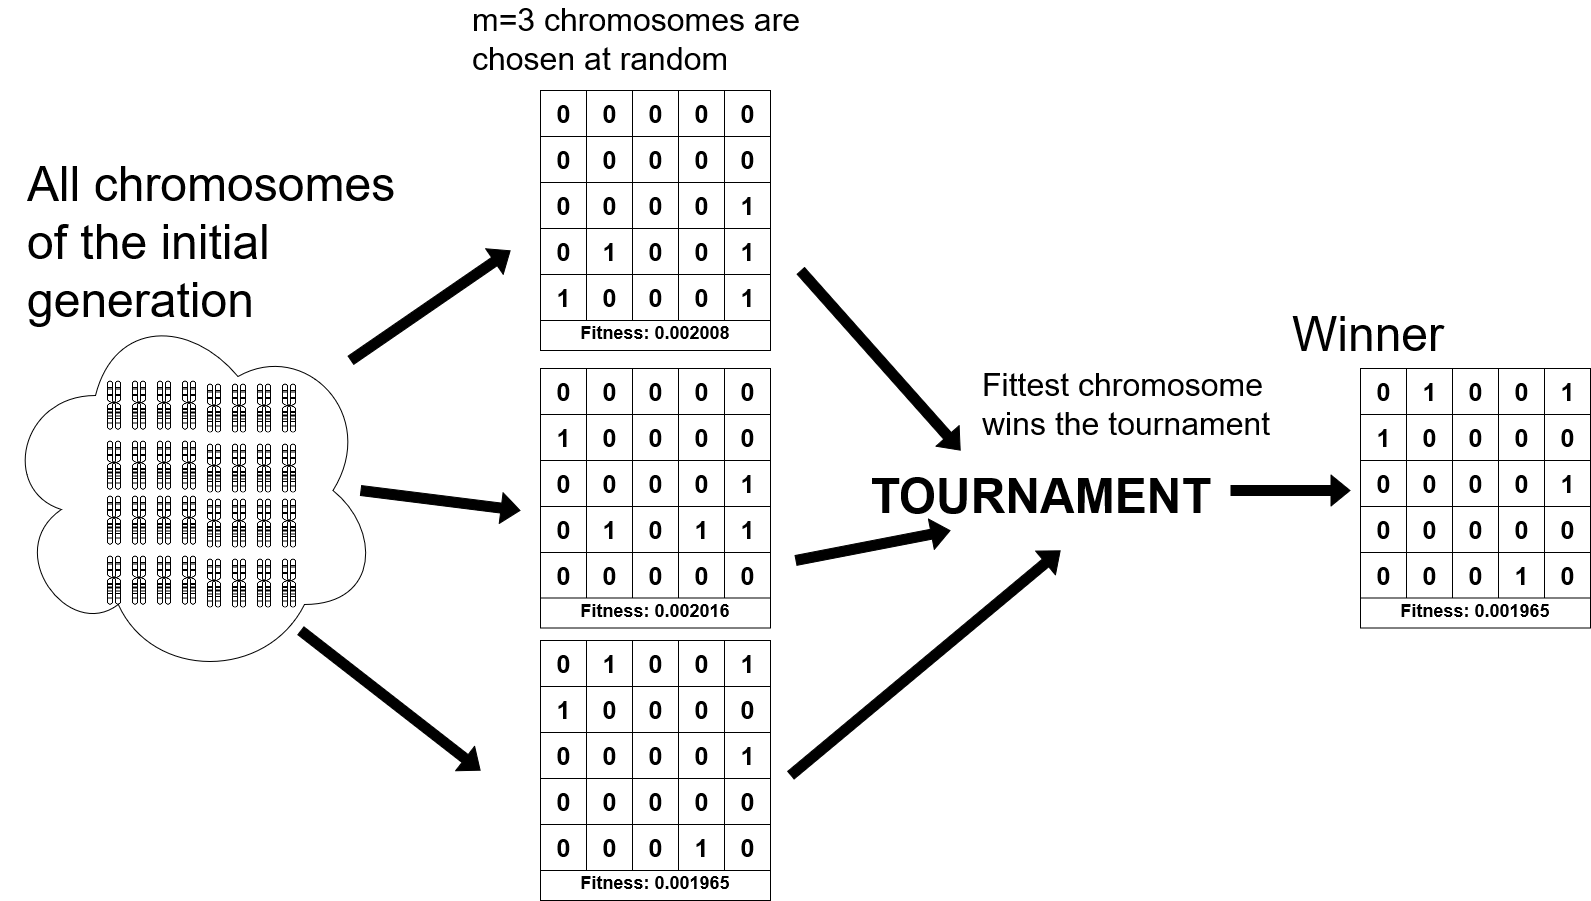
\includegraphics[width=\linewidth]{Figures/tournamentSmall.png}
        \caption{First Crossover of Generation 1}
        \label{tournamentSmall}
    \end{figure}
    
    For the first tournament, three chromosomes are chosen at random as competitors of the first tournament from the initial population. The chosen chromosomes were $P_{14}$, $P_{09}$ and $P_{54}$ with fitness values of 0.002008, 0.002016, and 0.001965 respectively. Since $P_{54}$ has the best fitness value, $P_{54}$ becomes the winner of the competition. The winner becomes part of the next generation and might be a parent for the crossover, see figure \ref{tournamentSmall}.

    After the tournament selection of the winner chromosomes the crossover step is done next. In figure 1 for example, Two random parents from the pool of the winner chromosomes performed a crossover using a random mask and produced two offspring. 
    
    \begin{figure}[h]
        \centering
        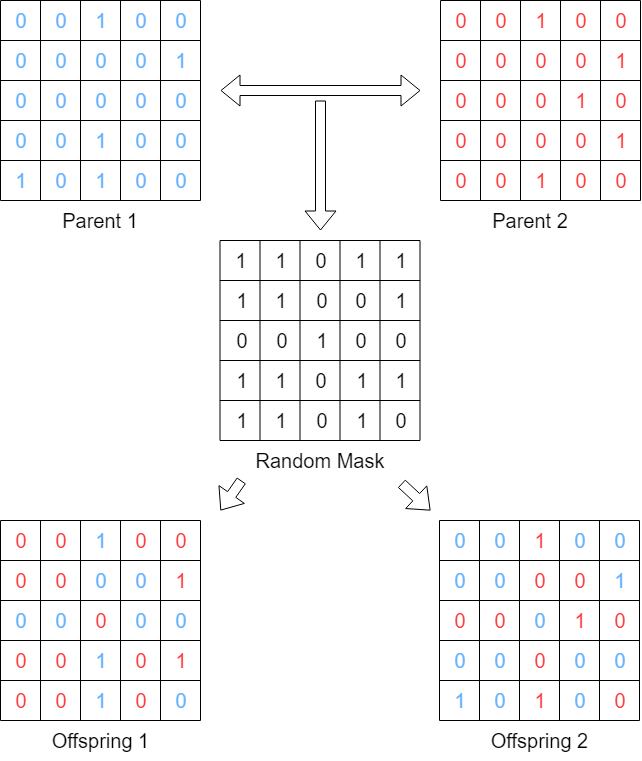
\includegraphics[width=100mm]{Figures/crossoverSmall.png}
        \caption{First Crossover of Generation 1}
        \label{fig:my_label}
    \end{figure}
    
    The crossover is done 35 times to produce enough offspring to fill in the next generation. The following rows of matrices shows the crossovers done in generation 1 where $Par_1$ and $Par_2$ are parents 1 and 2, $R$ is the random mask and $O_1$ and $O_2$ are the offspring 1 and 2.
    
    \singlespacing
    \fontsize{10}{12}\selectfont
    $$
        Par_{1} : \begin{bmatrix}
            0 & 0 & 1 & 0 & 0 \\
            0 & 0 & 0 & 0 & 1 \\
            0 & 0 & 0 & 0 & 0 \\
			0 & 0 & 1 & 0 & 0 \\
            1 & 0 & 1 & 0 & 0 
        \end{bmatrix}
        \;
         Par_{2} : \begin{bmatrix}
            0 & 0 & 1 & 0 & 0 \\
            0 & 0 & 0 & 0 & 1 \\
            0 & 0 & 0 & 1 & 0 \\
            0 & 0 & 0 & 0 & 1 \\
            0 & 0 & 1 & 0 & 0
        \end{bmatrix}
        \;
        R : \begin{bmatrix}
            1 & 1 & 0 & 1 & 1 \\
            1 & 1 & 0 & 0 & 1 \\
            0 & 0 & 1 & 0 & 0 \\
            1 & 1 & 0 & 1 & 1 \\
            1 & 1 & 0 & 1 & 0
        \end{bmatrix}
        \;
        O_{1} : \begin{bmatrix}
            0 & 0 & 1 & 0 & 0 \\
            0 & 0 & 0 & 0 & 1 \\
            0 & 0 & 0 & 0 & 0 \\
            0 & 0 & 1 & 0 & 1 \\
            0 & 0 & 1 & 0 & 0
        \end{bmatrix}
        \;
        O_{2} : \begin{bmatrix}
            0 & 0 & 1 & 0 & 0 \\
            0 & 0 & 0 & 0 & 1 \\
            0 & 0 & 0 & 1 & 0 \\
            0 & 0 & 0 & 0 & 0 \\
            1 & 0 & 1 & 0 & 0
        \end{bmatrix}
    $$
    $$
        Par_{1} : \begin{bmatrix}
            1 & 0 & 0 & 1 & 0 \\
            0 & 0 & 0 & 0 & 1 \\
            0 & 0 & 0 & 0 & 0 \\
			0 & 0 & 1 & 1 & 0 \\
            1 & 0 & 0 & 0 & 0 
        \end{bmatrix}
        \;
         Par_{2} : \begin{bmatrix}
            0 & 0 & 1 & 0 & 0 \\
            0 & 0 & 0 & 0 & 1 \\
            0 & 0 & 0 & 1 & 0 \\
            0 & 0 & 0 & 0 & 1 \\
            0 & 0 & 1 & 0 & 0
        \end{bmatrix}
        \;
        R : \begin{bmatrix}
            1 & 1 & 1 & 0 & 0 \\
            0 & 0 & 1 & 1 & 1 \\
            0 & 1 & 0 & 0 & 0 \\
            0 & 0 & 1 & 1 & 1 \\
            1 & 1 & 1 & 1 & 1
        \end{bmatrix}
        \;
        O_{1} : \begin{bmatrix}
            0 & 0 & 1 & 1 & 0 \\
            0 & 0 & 0 & 0 & 1 \\
            0 & 0 & 0 & 0 & 0 \\
            0 & 0 & 0 & 0 & 1 \\
            0 & 0 & 1 & 0 & 0
        \end{bmatrix}
        \;
        O_{2} : \begin{bmatrix}
            1 & 0 & 0 & 0 & 0 \\
            0 & 0 & 0 & 0 & 0 \\
            0 & 0 & 0 & 1 & 0 \\
            0 & 0 & 1 & 1 & 0 \\
            1 & 0 & 0 & 0 & 0
        \end{bmatrix}
    $$
     $$
        Par_{1} : \begin{bmatrix}
            0 & 1 & 0 & 0 & 0 \\
            0 & 1 & 1 & 0 & 0 \\
            0 & 0 & 0 & 0 & 0 \\
			0 & 0 & 0 & 0 & 1 \\
            1 & 0 & 0 & 0 & 0 
        \end{bmatrix}
        \;
        Par_{2} : \begin{bmatrix}
            0 & 0 & 0 & 0 & 0 \\
            1 & 0 & 0 & 0 & 0 \\
            0 & 0 & 0 & 0 & 0 \\
            0 & 0 & 1 & 0 & 0 \\
            0 & 1 & 0 & 1 & 1
        \end{bmatrix}
        \;
        R : \begin{bmatrix}
            0 & 0 & 0 & 0 & 1 \\
            1 & 1 & 1 & 1 & 1 \\
            0 & 1 & 1 & 1 & 0 \\
            1 & 1 & 1 & 0 & 1 \\
            1 & 0 & 1 & 1 & 0
        \end{bmatrix}
        \;
        O_{1} : \begin{bmatrix}
            0 & 1 & 0 & 0 & 0 \\
            1 & 0 & 0 & 0 & 0 \\
            0 & 0 & 0 & 0 & 0 \\
            0 & 0 & 1 & 0 & 0 \\
            0 & 0 & 0 & 1 & 0
        \end{bmatrix}
        \;
        O_{2} : \begin{bmatrix}
            0 & 0 & 0 & 0 & 0 \\
            0 & 1 & 1 & 0 & 0 \\
            0 & 0 & 0 & 0 & 0 \\
            0 & 0 & 0 & 0 & 1 \\
            1 & 1 & 0 & 0 & 1
        \end{bmatrix}
    $$   
     $$
        Par_{1} : \begin{bmatrix}
            0 & 0 & 0 & 0 & 1 \\
            1 & 0 & 0 & 0 & 0 \\
            0 & 0 & 0 & 0 & 0 \\
			0 & 0 & 1 & 0 & 1 \\
            0 & 0 & 0 & 1 & 0 
        \end{bmatrix}
        \;
        Par_{2} : \begin{bmatrix}
            0 & 1 & 1 & 0 & 0 \\
            0 & 0 & 0 & 1 & 0 \\
            1 & 0 & 0 & 0 & 0 \\
            0 & 0 & 1 & 0 & 0 \\
            0 & 0 & 0 & 0 & 0
        \end{bmatrix}
        \;
        R : \begin{bmatrix}
            0 & 1 & 1 & 0 & 1 \\
            1 & 0 & 1 & 0 & 0 \\
            0 & 0 & 1 & 1 & 0 \\
            1 & 1 & 0 & 1 & 0 \\
            0 & 0 & 1 & 1 & 0
        \end{bmatrix}
        \;
        O_{1} : \begin{bmatrix}
            0 & 1 & 1 & 0 & 0 \\
            0 & 0 & 0 & 0 & 0 \\
            0 & 0 & 0 & 0 & 0 \\
            0 & 0 & 1 & 0 & 1 \\
            0 & 0 & 0 & 0 & 0
        \end{bmatrix}
        \;
        O_{2} : \begin{bmatrix}
            0 & 0 & 0 & 0 & 1 \\
            1 & 0 & 0 & 1 & 0 \\
            1 & 0 & 0 & 0 & 0 \\
            0 & 0 & 1 & 0 & 0 \\
            0 & 0 & 0 & 1 & 0
        \end{bmatrix}
    $$ 
     $$
        Par_{1} : \begin{bmatrix}
            0 & 1 & 0 & 0 & 1 \\
            0 & 0 & 0 & 0 & 0 \\
            0 & 0 & 0 & 0 & 0 \\
			1 & 0 & 0 & 1 & 0 \\
            0 & 0 & 0 & 1 & 0 
        \end{bmatrix}
        \;
        Par_{2} : \begin{bmatrix}
            0 & 0 & 0 & 0 & 0 \\
            1 & 1 & 0 & 0 & 1 \\
            0 & 0 & 0 & 0 & 0 \\
            0 & 0 & 0 & 0 & 0 \\
            1 & 0 & 0 & 0 & 1
        \end{bmatrix}
        \;
        R : \begin{bmatrix}
            1 & 0 & 1 & 1 & 1 \\
            1 & 1 & 0 & 0 & 1 \\
            1 & 1 & 0 & 1 & 1 \\
            1 & 1 & 1 & 1 & 0 \\
            1 & 0 & 1 & 0 & 0
        \end{bmatrix}
        \;
        O_{1} : \begin{bmatrix}
            0 & 1 & 0 & 0 & 0 \\
            1 & 1 & 0 & 0 & 1 \\
            0 & 0 & 0 & 0 & 0 \\
            0 & 0 & 0 & 0 & 0 \\
            1 & 0 & 0 & 1 & 0
        \end{bmatrix}
        \;
        O_{2} : \begin{bmatrix}
            0 & 0 & 0 & 0 & 1 \\
            0 & 0 & 0 & 0 & 0 \\
            0 & 0 & 0 & 0 & 0 \\
            1 & 0 & 0 & 1 & 0 \\
            0 & 0 & 0 & 0 & 1
        \end{bmatrix}
    $$ 
     $$
        Par_{1} : \begin{bmatrix}
            1 & 0 & 0 & 0 & 0 \\
            0 & 0 & 0 & 0 & 0 \\
            0 & 1 & 0 & 0 & 0 \\
			0 & 0 & 0 & 0 & 0 \\
            1 & 0 & 0 & 1 & 1 
        \end{bmatrix}
        \;
        Par_{2} : \begin{bmatrix}
            0 & 0 & 0 & 1 & 0 \\
            0 & 0 & 0 & 0 & 1 \\
            1 & 0 & 0 & 1 & 0 \\
            0 & 0 & 0 & 0 & 0 \\
            0 & 0 & 0 & 1 & 0
        \end{bmatrix}
        \;
        R : \begin{bmatrix}
            0 & 1 & 1 & 0 & 1 \\
            1 & 1 & 0 & 1 & 0 \\
            0 & 0 & 1 & 0 & 0 \\
            0 & 1 & 1 & 1 & 0 \\
            1 & 1 & 0 & 1 & 0
        \end{bmatrix}
        \;
        O_{1} : \begin{bmatrix}
            1 & 0 & 0 & 0 & 0 \\
            0 & 0 & 0 & 0 & 0 \\
            0 & 1 & 0 & 0 & 0 \\
            0 & 0 & 0 & 0 & 0 \\
            0 & 0 & 0 & 1 & 1
        \end{bmatrix}
        \;
        O_{2} : \begin{bmatrix}
            0 & 0 & 0 & 1 & 0 \\
            0 & 0 & 0 & 0 & 1 \\
            1 & 0 & 0 & 1 & 0 \\
            0 & 0 & 0 & 0 & 0 \\
            1 & 0 & 0 & 1 & 0
        \end{bmatrix}
    $$ 
     $$
        Par_{1} : \begin{bmatrix}
            0 & 0 & 1 & 0 & 0 \\
            0 & 0 & 0 & 0 & 1 \\
            0 & 0 & 0 & 1 & 0 \\
			0 & 0 & 0 & 0 & 1 \\
            0 & 0 & 1 & 0 & 0 
        \end{bmatrix}
        \;
        Par_{2} : \begin{bmatrix}
            0 & 1 & 0 & 0 & 1 \\
            0 & 0 & 0 & 0 & 0 \\
            0 & 0 & 1 & 0 & 0 \\
            0 & 0 & 0 & 0 & 0 \\
            1 & 0 & 0 & 0 & 1
        \end{bmatrix}
        \;
        R : \begin{bmatrix}
            0 & 1 & 1 & 0 & 0 \\
            1 & 0 & 0 & 1 & 0 \\
            1 & 0 & 1 & 1 & 1 \\
            1 & 1 & 0 & 0 & 1 \\
            1 & 0 & 0 & 1 & 1
        \end{bmatrix}
        \;
        O_{1} : \begin{bmatrix}
            0 & 1 & 0 & 0 & 0 \\
            0 & 0 & 0 & 0 & 1 \\
            0 & 0 & 0 & 1 & 0 \\
            0 & 0 & 0 & 0 & 0 \\
            1 & 0 & 1 & 0 & 1
        \end{bmatrix}
        \;
        O_{2} : \begin{bmatrix}
            0 & 0 & 1 & 0 & 1 \\
            0 & 0 & 0 & 0 & 0 \\
            0 & 0 & 0 & 1 & 0 \\
            0 & 0 & 0 & 0 & 1 \\
            0 & 0 & 0 & 0 & 0
        \end{bmatrix}
    $$ 
     $$
        Par_{1} : \begin{bmatrix}
            0 & 1 & 0 & 0 & 0 \\
            0 & 0 & 0 & 0 & 0 \\
            1 & 1 & 0 & 0 & 0 \\
			0 & 0 & 0 & 0 & 0 \\
            0 & 0 & 1 & 0 & 1 
        \end{bmatrix}
        \;
        Par_{2} : \begin{bmatrix}
            0 & 1 & 0 & 0 & 1 \\
            0 & 0 & 0 & 0 & 0 \\
            0 & 0 & 1 & 0 & 0 \\
            0 & 0 & 0 & 0 & 0 \\
            1 & 0 & 0 & 0 & 1
        \end{bmatrix}
        \;
        R : \begin{bmatrix}
            0 & 0 & 0 & 1 & 0 \\
            0 & 0 & 0 & 0 & 1 \\
            0 & 1 & 0 & 1 & 0 \\
            1 & 1 & 0 & 0 & 1 \\
            0 & 1 & 1 & 1 & 0
        \end{bmatrix}
        \;
        O_{1} : \begin{bmatrix}
            0 & 1 & 0 & 0 & 0 \\
            0 & 0 & 0 & 0 & 0 \\
            1 & 0 & 0 & 0 & 0 \\
            0 & 0 & 0 & 0 & 0 \\
            0 & 0 & 0 & 0 & 1
        \end{bmatrix}
        \;
        O_{2} : \begin{bmatrix}
            0 & 1 & 0 & 0 & 1 \\
            0 & 0 & 0 & 0 & 0 \\
            0 & 1 & 1 & 0 & 0 \\
            0 & 0 & 0 & 0 & 0 \\
            1 & 0 & 1 & 0 & 1
        \end{bmatrix}
    $$ 
     $$
        Par_{1} : \begin{bmatrix}
            1 & 0 & 0 & 0 & 0 \\
            0 & 0 & 0 & 0 & 0 \\
            0 & 1 & 0 & 0 & 0 \\
			0 & 0 & 0 & 0 & 0 \\
            1 & 0 & 0 & 1 & 1 
        \end{bmatrix}
        \;
        Par_{2} : \begin{bmatrix}
            0 & 0 & 0 & 1 & 0 \\
            0 & 0 & 0 & 0 & 1 \\
            1 & 0 & 0 & 1 & 0 \\
            0 & 0 & 0 & 0 & 0 \\
            0 & 0 & 0 & 1 & 0
        \end{bmatrix}
        \;
        R : \begin{bmatrix}
            1 & 1 & 0 & 0 & 0 \\
            1 & 1 & 0 & 1 & 1 \\
            0 & 0 & 0 & 0 & 0 \\
            0 & 1 & 0 & 1 & 1 \\
            1 & 0 & 0 & 1 & 0
        \end{bmatrix}
        \;
        O_{1} : \begin{bmatrix}
            0 & 0 & 0 & 0 & 0 \\
            0 & 0 & 0 & 0 & 1 \\
            0 & 1 & 0 & 0 & 0 \\
            0 & 0 & 0 & 0 & 0 \\
            0 & 0 & 0 & 1 & 1
        \end{bmatrix}
        \;
        O_{2} : \begin{bmatrix}
            1 & 0 & 0 & 1 & 0 \\
            0 & 0 & 0 & 0 & 0 \\
            1 & 0 & 0 & 1 & 0 \\
            0 & 0 & 0 & 0 & 0 \\
            1 & 0 & 0 & 1 & 0
        \end{bmatrix}
    $$ 
     $$
        Par_{1} : \begin{bmatrix}
            0 & 0 & 0 & 0 & 1 \\
            1 & 0 & 0 & 0 & 0 \\
            0 & 0 & 0 & 0 & 0 \\
			0 & 0 & 1 & 0 & 1 \\
            0 & 0 & 0 & 1 & 0 
        \end{bmatrix}
        \;
        Par_{2} : \begin{bmatrix}
            0 & 0 & 0 & 0 & 0 \\
            0 & 0 & 0 & 1 & 0 \\
            0 & 0 & 0 & 0 & 1 \\
            0 & 0 & 0 & 1 & 0 \\
            1 & 0 & 0 & 0 & 1
        \end{bmatrix}
        \;
        R : \begin{bmatrix}
            0 & 1 & 1 & 1 & 1 \\
            0 & 1 & 0 & 1 & 1 \\
            0 & 1 & 1 & 1 & 0 \\
            1 & 0 & 1 & 1 & 0 \\
            1 & 1 & 1 & 1 & 0
        \end{bmatrix}
        \;
        O_{1} : \begin{bmatrix}
            0 & 0 & 0 & 0 & 0 \\
            1 & 0 & 0 & 1 & 0 \\
            0 & 0 & 0 & 0 & 0 \\
            0 & 0 & 0 & 1 & 1 \\
            1 & 0 & 0 & 0 & 0
        \end{bmatrix}
        \;
        O_{2} : \begin{bmatrix}
            0 & 0 & 0 & 0 & 1 \\
            0 & 0 & 0 & 0 & 0 \\
            0 & 0 & 0 & 0 & 1 \\
            0 & 0 & 1 & 0 & 0 \\
            0 & 0 & 0 & 1 & 1
        \end{bmatrix}
    $$ 
     $$
        Par_{1} : \begin{bmatrix}
            0 & 0 & 0 & 0 & 0 \\
            0 & 1 & 0 & 1 & 0 \\
            1 & 1 & 0 & 0 & 0 \\
			0 & 0 & 1 & 0 & 0 \\
            0 & 0 & 0 & 0 & 0 
        \end{bmatrix}
        \;
        Par_{2} : \begin{bmatrix}
            0 & 1 & 0 & 0 & 0 \\
            0 & 0 & 0 & 0 & 0 \\
            1 & 1 & 0 & 0 & 0 \\
            0 & 0 & 0 & 0 & 0 \\
            0 & 0 & 1 & 0 & 1
        \end{bmatrix}
        \;
        R : \begin{bmatrix}
            1 & 0 & 1 & 1 & 1 \\
            0 & 1 & 1 & 1 & 1 \\
            1 & 0 & 1 & 0 & 1 \\
            0 & 1 & 0 & 1 & 0 \\
            0 & 0 & 0 & 1 & 0
        \end{bmatrix}
        \;
        O_{1} : \begin{bmatrix}
            0 & 0 & 0 & 0 & 0 \\
            0 & 0 & 0 & 0 & 0 \\
            1 & 1 & 0 & 0 & 0 \\
            0 & 0 & 1 & 0 & 0 \\
            0 & 0 & 0 & 0 & 0
        \end{bmatrix}
        \;
        O_{2} : \begin{bmatrix}
            0 & 1 & 0 & 0 & 0 \\
            0 & 1 & 0 & 1 & 0 \\
            1 & 1 & 0 & 0 & 0 \\
            0 & 0 & 0 & 0 & 0 \\
            0 & 0 & 1 & 0 & 1
        \end{bmatrix}
    $$ 
     $$
        Par_{1} : \begin{bmatrix}
            0 & 1 & 0 & 0 & 0 \\
            0 & 0 & 0 & 0 & 1 \\
            0 & 1 & 0 & 0 & 0 \\
			0 & 0 & 0 & 1 & 0 \\
            0 & 0 & 1 & 0 & 0 
        \end{bmatrix}
        \;
        Par_{2} : \begin{bmatrix}
            0 & 0 & 0 & 0 & 1 \\
            1 & 0 & 0 & 0 & 0 \\
            0 & 0 & 0 & 1 & 0 \\
            0 & 0 & 0 & 1 & 0 \\
            1 & 0 & 0 & 0 & 0
        \end{bmatrix}
        \;
        R : \begin{bmatrix}
            0 & 0 & 1 & 0 & 0 \\
            0 & 0 & 1 & 1 & 1 \\
            1 & 0 & 0 & 1 & 1 \\
            0 & 1 & 1 & 0 & 1 \\
            0 & 0 & 0 & 0 & 1
        \end{bmatrix}
        \;
        O_{1} : \begin{bmatrix}
            0 & 1 & 0 & 0 & 0 \\
            0 & 0 & 0 & 0 & 0 \\
            0 & 1 & 0 & 1 & 0 \\
            0 & 0 & 0 & 1 & 0 \\
            0 & 0 & 1 & 0 & 0
        \end{bmatrix}
        \;
        O_{2} : \begin{bmatrix}
            0 & 0 & 0 & 0 & 1 \\
            1 & 0 & 0 & 0 & 1 \\
            0 & 0 & 0 & 0 & 0 \\
            0 & 0 & 0 & 1 & 0 \\
            1 & 0 & 0 & 0 & 0
        \end{bmatrix}
    $$ 
     $$
        Par_{1} : \begin{bmatrix}
            0 & 0 & 0 & 0 & 0 \\
            0 & 0 & 0 & 1 & 0 \\
            0 & 0 & 0 & 0 & 1 \\
			0 & 0 & 0 & 1 & 0 \\
            1 & 0 & 0 & 0 & 1 
        \end{bmatrix}
        \;
        Par_{2} : \begin{bmatrix}
            0 & 0 & 0 & 0 & 1 \\
            1 & 0 & 0 & 0 & 0 \\
            0 & 0 & 0 & 0 & 0 \\
            0 & 0 & 1 & 0 & 1 \\
            0 & 0 & 0 & 1 & 0
        \end{bmatrix}
        \;
        R : \begin{bmatrix}
            1 & 0 & 1 & 0 & 0 \\
            0 & 1 & 0 & 0 & 1 \\
            0 & 0 & 1 & 0 & 0 \\
            1 & 1 & 0 & 1 & 0 \\
            0 & 1 & 0 & 0 & 0
        \end{bmatrix}
        \;
        O_{1} : \begin{bmatrix}
            0 & 0 & 0 & 0 & 0 \\
            0 & 0 & 0 & 1 & 0 \\
            0 & 0 & 0 & 0 & 1 \\
            0 & 0 & 0 & 0 & 0 \\
            1 & 0 & 0 & 0 & 1
        \end{bmatrix}
        \;
        O_{2} : \begin{bmatrix}
            0 & 0 & 0 & 0 & 1 \\
            1 & 0 & 0 & 0 & 0 \\
            0 & 0 & 0 & 0 & 0 \\
            0 & 0 & 1 & 1 & 1 \\
            0 & 0 & 0 & 1 & 0
        \end{bmatrix}
    $$ 
     $$
        Par_{1} : \begin{bmatrix}
            1 & 0 & 0 & 0 & 0 \\
            1 & 0 & 0 & 0 & 1 \\
            0 & 0 & 0 & 0 & 0 \\
			0 & 0 & 0 & 1 & 0 \\
            1 & 0 & 0 & 0 & 0 
        \end{bmatrix}
        \;
        Par_{2} : \begin{bmatrix}
            1 & 0 & 0 & 0 & 0 \\
            0 & 0 & 0 & 0 & 0 \\
            0 & 1 & 0 & 0 & 0 \\
            0 & 0 & 0 & 0 & 0 \\
            1 & 0 & 0 & 1 & 1
        \end{bmatrix}
        \;
        R : \begin{bmatrix}
            0 & 1 & 0 & 0 & 0 \\
            1 & 1 & 1 & 0 & 0 \\
            0 & 1 & 0 & 1 & 1 \\
            1 & 1 & 0 & 0 & 1 \\
            0 & 0 & 1 & 0 & 1
        \end{bmatrix}
        \;
        O_{1} : \begin{bmatrix}
            1 & 0 & 0 & 0 & 0 \\
            0 & 0 & 0 & 0 & 1 \\
            0 & 1 & 0 & 0 & 0 \\
            0 & 0 & 0 & 1 & 0 \\
            1 & 0 & 0 & 0 & 1
        \end{bmatrix}
        \;
        O_{2} : \begin{bmatrix}
            1 & 0 & 0 & 0 & 0 \\
            1 & 0 & 0 & 0 & 0 \\
            0 & 0 & 0 & 0 & 0 \\
            0 & 0 & 0 & 0 & 0 \\
            1 & 0 & 0 & 1 & 0
        \end{bmatrix}
    $$ 
     $$
        Par_{1} : \begin{bmatrix}
            0 & 1 & 0 & 0 & 0 \\
            0 & 1 & 1 & 0 & 0 \\
            0 & 0 & 0 & 0 & 0 \\
			0 & 0 & 0 & 0 & 1 \\
            1 & 0 & 0 & 0 & 0 
        \end{bmatrix}
        \;
        Par_{2} : \begin{bmatrix}
            0 & 1 & 0 & 0 & 1 \\
            0 & 0 & 0 & 0 & 0 \\
            0 & 0 & 0 & 0 & 0 \\
            1 & 0 & 0 & 1 & 0 \\
            0 & 0 & 0 & 1 & 0
        \end{bmatrix}
        \;
        R : \begin{bmatrix}
            1 & 1 & 0 & 1 & 1 \\
            0 & 1 & 0 & 0 & 1 \\
            0 & 0 & 0 & 1 & 0 \\
            1 & 1 & 0 & 0 & 0 \\
            1 & 0 & 1 & 0 & 0
        \end{bmatrix}
        \;
        O_{1} : \begin{bmatrix}
            0 & 1 & 0 & 0 & 1 \\
            0 & 0 & 1 & 0 & 0 \\
            0 & 0 & 0 & 0 & 0 \\
            1 & 0 & 0 & 0 & 1 \\
            0 & 0 & 0 & 0 & 0
        \end{bmatrix}
        \;
        O_{2} : \begin{bmatrix}
            0 & 1 & 0 & 0 & 0 \\
            0 & 1 & 0 & 0 & 0 \\
            0 & 0 & 0 & 0 & 0 \\
            0 & 0 & 0 & 1 & 0 \\
            1 & 0 & 0 & 1 & 0
        \end{bmatrix}
    $$ 
     $$
        Par_{1} : \begin{bmatrix}
            0 & 0 & 0 & 0 & 1 \\
            1 & 0 & 0 & 0 & 0 \\
            0 & 0 & 0 & 0 & 0 \\
			0 & 0 & 1 & 0 & 1 \\
            0 & 0 & 0 & 1 & 0 
        \end{bmatrix}
        \;
        Par_{2} : \begin{bmatrix}
            0 & 1 & 0 & 0 & 0 \\
            0 & 0 & 0 & 0 & 0 \\
            1 & 1 & 0 & 0 & 0 \\
            0 & 0 & 0 & 0 & 0 \\
            0 & 0 & 1 & 0 & 1
        \end{bmatrix}
        \;
        R : \begin{bmatrix}
            1 & 1 & 0 & 0 & 0 \\
            0 & 1 & 0 & 0 & 1 \\
            0 & 1 & 0 & 1 & 0 \\
            0 & 0 & 0 & 0 & 0 \\
            1 & 1 & 0 & 0 & 0
        \end{bmatrix}
        \;
        O_{1} : \begin{bmatrix}
            0 & 1 & 0 & 0 & 1 \\
            1 & 0 & 0 & 0 & 0 \\
            0 & 1 & 0 & 0 & 0 \\
            0 & 0 & 1 & 0 & 1 \\
            0 & 0 & 0 & 1 & 0
        \end{bmatrix}
        \;
        O_{2} : \begin{bmatrix}
            0 & 0 & 0 & 0 & 0 \\
            0 & 0 & 0 & 0 & 0 \\
            1 & 0 & 0 & 0 & 0 \\
            0 & 0 & 0 & 0 & 0 \\
            0 & 0 & 1 & 0 & 1
        \end{bmatrix}
    $$ 
     $$
        Par_{1} : \begin{bmatrix}
            0 & 1 & 1 & 0 & 0 \\
            0 & 0 & 0 & 1 & 0 \\
            1 & 0 & 0 & 0 & 0 \\
			0 & 0 & 1 & 0 & 0 \\
            0 & 0 & 0 & 0 & 0 
        \end{bmatrix}
        \;
        Par_{2} : \begin{bmatrix}
            1 & 0 & 0 & 1 & 0 \\
            0 & 0 & 0 & 0 & 0 \\
            0 & 0 & 0 & 0 & 0 \\
            0 & 0 & 1 & 1 & 0 \\
            1 & 0 & 0 & 0 & 0
        \end{bmatrix}
        \;
        R : \begin{bmatrix}
            0 & 0 & 0 & 1 & 0 \\
            0 & 0 & 0 & 0 & 0 \\
            1 & 1 & 1 & 0 & 0 \\
            1 & 1 & 1 & 1 & 1 \\
            0 & 0 & 0 & 1 & 0
        \end{bmatrix}
        \;
        O_{1} : \begin{bmatrix}
            0 & 1 & 1 & 1 & 0 \\
            0 & 0 & 0 & 1 & 0 \\
            0 & 0 & 0 & 0 & 0 \\
            0 & 0 & 1 & 1 & 0 \\
            0 & 0 & 0 & 0 & 0
        \end{bmatrix}
        \;
        O_{2} : \begin{bmatrix}
            1 & 0 & 0 & 0 & 0 \\
            0 & 0 & 0 & 0 & 0 \\
            1 & 0 & 0 & 0 & 0 \\
            0 & 0 & 1 & 0 & 0 \\
            1 & 0 & 0 & 0 & 0
        \end{bmatrix}
    $$ 
     $$
        Par_{1} : \begin{bmatrix}
            1 & 0 & 0 & 0 & 0 \\
            0 & 0 & 1 & 1 & 0 \\
            0 & 1 & 0 & 0 & 0 \\
			0 & 0 & 0 & 0 & 0 \\
            0 & 0 & 1 & 0 & 0 
        \end{bmatrix}
        \;
        Par_{2} : \begin{bmatrix}
            0 & 1 & 1 & 0 & 0 \\
            0 & 0 & 0 & 1 & 0 \\
            1 & 0 & 0 & 0 & 0 \\
            0 & 0 & 1 & 0 & 0 \\
            0 & 0 & 0 & 0 & 0
        \end{bmatrix}
        \;
        R : \begin{bmatrix}
            1 & 1 & 0 & 0 & 1 \\
            1 & 0 & 0 & 1 & 1 \\
            0 & 1 & 0 & 1 & 0 \\
            1 & 1 & 0 & 1 & 0 \\
            1 & 1 & 0 & 1 & 0
        \end{bmatrix}
        \;
        O_{1} : \begin{bmatrix}
            0 & 1 & 0 & 0 & 0 \\
            0 & 0 & 1 & 1 & 0 \\
            0 & 0 & 0 & 0 & 0 \\
            0 & 0 & 0 & 0 & 0 \\
            0 & 0 & 1 & 0 & 0
        \end{bmatrix}
        \;
        O_{2} : \begin{bmatrix}
            1 & 0 & 1 & 0 & 0 \\
            0 & 0 & 0 & 1 & 0 \\
            1 & 1 & 0 & 0 & 0 \\
            0 & 0 & 1 & 0 & 0 \\
            0 & 0 & 0 & 0 & 0
        \end{bmatrix}
    $$ 
     $$
        Par_{1} : \begin{bmatrix}
            0 & 1 & 0 & 1 & 0 \\
            0 & 0 & 0 & 0 & 0 \\
            0 & 1 & 0 & 0 & 0 \\
			0 & 0 & 1 & 0 & 0 \\
            0 & 0 & 0 & 0 & 1 
        \end{bmatrix}
        \;
        Par_{2} : \begin{bmatrix}
            0 & 0 & 0 & 0 & 0 \\
            0 & 0 & 0 & 0 & 1 \\
            0 & 0 & 0 & 1 & 0 \\
            0 & 0 & 0 & 0 & 0 \\
            1 & 1 & 0 & 0 & 1
        \end{bmatrix}
        \;
        R : \begin{bmatrix}
            1 & 1 & 0 & 0 & 0 \\
            0 & 0 & 0 & 0 & 0 \\
            1 & 1 & 0 & 1 & 0 \\
            0 & 0 & 0 & 1 & 1 \\
            0 & 0 & 1 & 1 & 0
        \end{bmatrix}
        \;
        O_{1} : \begin{bmatrix}
            0 & 0 & 0 & 1 & 0 \\
            0 & 0 & 0 & 0 & 0 \\
            0 & 0 & 0 & 1 & 0 \\
            0 & 0 & 1 & 0 & 0 \\
            0 & 0 & 0 & 0 & 1
        \end{bmatrix}
        \;
        O_{2} : \begin{bmatrix}
            0 & 1 & 0 & 0 & 0 \\
            0 & 0 & 0 & 0 & 1 \\
            0 & 1 & 0 & 0 & 0 \\
            0 & 0 & 0 & 0 & 0 \\
            1 & 1 & 0 & 0 & 1
        \end{bmatrix}
    $$ 
     $$
        Par_{1} : \begin{bmatrix}
            0 & 0 & 0 & 1 & 0 \\
            0 & 0 & 1 & 0 & 0 \\
            0 & 0 & 0 & 0 & 1 \\
			0 & 0 & 0 & 0 & 0 \\
            1 & 0 & 0 & 1 & 0 
        \end{bmatrix}
        \;
        Par_{2} : \begin{bmatrix}
            0 & 0 & 0 & 1 & 0 \\
            0 & 0 & 0 & 0 & 1 \\
            1 & 0 & 0 & 1 & 0 \\
            0 & 0 & 0 & 0 & 0 \\
            0 & 0 & 0 & 1 & 0
        \end{bmatrix}
        \;
        R : \begin{bmatrix}
            1 & 1 & 1 & 1 & 1 \\
            1 & 1 & 0 & 1 & 0 \\
            1 & 0 & 0 & 1 & 0 \\
            0 & 0 & 0 & 0 & 0 \\
            1 & 0 & 0 & 0 & 0
        \end{bmatrix}
        \;
        O_{1} : \begin{bmatrix}
            0 & 0 & 0 & 1 & 0 \\
            0 & 0 & 1 & 0 & 0 \\
            1 & 0 & 0 & 1 & 1 \\
            0 & 0 & 0 & 0 & 0 \\
            0 & 0 & 0 & 1 & 0
        \end{bmatrix}
        \;
        O_{2} : \begin{bmatrix}
            0 & 0 & 0 & 1 & 0 \\
            0 & 0 & 0 & 0 & 1 \\
            0 & 0 & 0 & 0 & 0 \\
            0 & 0 & 0 & 0 & 0 \\
            1 & 0 & 0 & 1 & 0
        \end{bmatrix}
    $$ 
     $$
        Par_{1} : \begin{bmatrix}
            0 & 1 & 0 & 1 & 0 \\
            0 & 0 & 0 & 0 & 0 \\
            0 & 1 & 0 & 0 & 0 \\
			0 & 0 & 1 & 0 & 0 \\
            0 & 0 & 0 & 0 & 1 
        \end{bmatrix}
        \;
        Par_{2} : \begin{bmatrix}
            0 & 0 & 1 & 0 & 0 \\
            0 & 0 & 0 & 0 & 1 \\
            0 & 0 & 0 & 0 & 0 \\
            0 & 0 & 1 & 0 & 0 \\
            1 & 0 & 1 & 0 & 0
        \end{bmatrix}
        \;
        R : \begin{bmatrix}
            1 & 0 & 0 & 0 & 1 \\
            0 & 1 & 0 & 1 & 0 \\
            0 & 0 & 0 & 1 & 1 \\
            0 & 0 & 0 & 1 & 1 \\
            1 & 0 & 0 & 1 & 0
        \end{bmatrix}
        \;
        O_{1} : \begin{bmatrix}
            0 & 1 & 0 & 1 & 0 \\
            0 & 0 & 0 & 0 & 0 \\
            0 & 1 & 0 & 0 & 0 \\
            0 & 0 & 1 & 0 & 0 \\
            1 & 0 & 0 & 0 & 1
        \end{bmatrix}
        \;
        O_{2} : \begin{bmatrix}
            0 & 0 & 1 & 0 & 0 \\
            0 & 0 & 0 & 0 & 1 \\
            0 & 0 & 0 & 0 & 0 \\
            0 & 0 & 1 & 0 & 0 \\
            0 & 0 & 1 & 0 & 0
        \end{bmatrix}
    $$ 
     $$
        Par_{1} : \begin{bmatrix}
            0 & 1 & 0 & 1 & 0 \\
            0 & 0 & 0 & 1 & 0 \\
            0 & 0 & 0 & 0 & 0 \\
			1 & 0 & 0 & 0 & 0 \\
            0 & 0 & 1 & 0 & 0 
        \end{bmatrix}
        \;
        Par_{2} : \begin{bmatrix}
            0 & 1 & 0 & 1 & 0 \\
            0 & 0 & 0 & 1 & 0 \\
            0 & 0 & 0 & 0 & 0 \\
            1 & 0 & 0 & 0 & 0 \\
            0 & 0 & 1 & 0 & 0
        \end{bmatrix}
        \;
        R : \begin{bmatrix}
            0 & 1 & 0 & 1 & 0 \\
            1 & 0 & 1 & 1 & 0 \\
            1 & 1 & 1 & 1 & 1 \\
            1 & 0 & 0 & 1 & 0 \\
            1 & 1 & 1 & 1 & 0
        \end{bmatrix}
        \;
        O_{1} : \begin{bmatrix}
            0 & 1 & 0 & 1 & 0 \\
            0 & 0 & 0 & 1 & 0 \\
            0 & 0 & 0 & 0 & 0 \\
            1 & 0 & 0 & 0 & 0 \\
            0 & 0 & 1 & 0 & 0
        \end{bmatrix}
        \;
        O_{2} : \begin{bmatrix}
            0 & 1 & 0 & 1 & 0 \\
            0 & 0 & 0 & 1 & 0 \\
            0 & 0 & 0 & 0 & 0 \\
            1 & 0 & 0 & 0 & 0 \\
            0 & 0 & 1 & 0 & 0
        \end{bmatrix}
    $$ 
     $$
        Par_{1} : \begin{bmatrix}
            0 & 1 & 0 & 1 & 0 \\
            0 & 0 & 0 & 0 & 0 \\
            0 & 1 & 0 & 0 & 0 \\
			0 & 0 & 1 & 0 & 0 \\
            0 & 0 & 0 & 0 & 1 
        \end{bmatrix}
        \;
        Par_{2} : \begin{bmatrix}
            1 & 0 & 0 & 1 & 0 \\
            0 & 0 & 0 & 0 & 0 \\
            0 & 0 & 0 & 0 & 0 \\
            0 & 0 & 1 & 1 & 0 \\
            1 & 0 & 0 & 0 & 0
        \end{bmatrix}
        \;
        R : \begin{bmatrix}
            1 & 1 & 1 & 1 & 1 \\
            1 & 1 & 1 & 1 & 1 \\
            0 & 0 & 1 & 1 & 0 \\
            0 & 1 & 1 & 0 & 1 \\
            1 & 0 & 0 & 1 & 1
        \end{bmatrix}
        \;
        O_{1} : \begin{bmatrix}
            1 & 0 & 0 & 1 & 0 \\
            0 & 0 & 0 & 0 & 0 \\
            0 & 1 & 0 & 0 & 0 \\
            0 & 0 & 1 & 0 & 0 \\
            1 & 0 & 0 & 0 & 0
        \end{bmatrix}
        \;
        O_{2} : \begin{bmatrix}
            0 & 1 & 0 & 1 & 0 \\
            0 & 0 & 0 & 0 & 0 \\
            0 & 0 & 0 & 0 & 0 \\
            0 & 0 & 1 & 1 & 0 \\
            0 & 0 & 0 & 0 & 1
        \end{bmatrix}
    $$ 
     $$
        Par_{1} : \begin{bmatrix}
            0 & 0 & 0 & 0 & 0 \\
            1 & 0 & 0 & 0 & 0 \\
            0 & 0 & 0 & 0 & 1 \\
			0 & 1 & 0 & 0 & 0 \\
            0 & 1 & 0 & 0 & 1 
        \end{bmatrix}
        \;
        Par_{2} : \begin{bmatrix}
            0 & 1 & 0 & 0 & 0 \\
            0 & 1 & 1 & 0 & 0 \\
            0 & 0 & 0 & 0 & 0 \\
            0 & 0 & 0 & 0 & 1 \\
            1 & 0 & 0 & 0 & 0
        \end{bmatrix}
        \;
        R : \begin{bmatrix}
            0 & 0 & 1 & 1 & 1 \\
            1 & 1 & 0 & 0 & 0 \\
            0 & 1 & 1 & 0 & 0 \\
            1 & 1 & 0 & 1 & 1 \\
            1 & 0 & 1 & 0 & 0
        \end{bmatrix}
        \;
        O_{1} : \begin{bmatrix}
            0 & 0 & 0 & 0 & 0 \\
            0 & 1 & 0 & 0 & 0 \\
            0 & 0 & 0 & 0 & 1 \\
            0 & 0 & 0 & 0 & 1 \\
            1 & 1 & 0 & 0 & 1
        \end{bmatrix}
        \;
        O_{2} : \begin{bmatrix}
            0 & 1 & 0 & 0 & 0 \\
            1 & 0 & 1 & 0 & 0 \\
            0 & 0 & 0 & 0 & 0 \\
            0 & 1 & 0 & 0 & 0 \\
            0 & 0 & 0 & 0 & 0
        \end{bmatrix}
    $$ 
     $$
        Par_{1} : \begin{bmatrix}
            0 & 0 & 0 & 0 & 1 \\
            1 & 0 & 0 & 0 & 0 \\
            0 & 0 & 0 & 1 & 0 \\
			0 & 0 & 0 & 1 & 0 \\
            1 & 0 & 0 & 0 & 0 
        \end{bmatrix}
        \;
        Par_{2} : \begin{bmatrix}
            0 & 0 & 0 & 0 & 1 \\
            1 & 0 & 0 & 0 & 0 \\
            0 & 0 & 0 & 1 & 0 \\
            0 & 0 & 0 & 1 & 0 \\
            1 & 0 & 0 & 0 & 0
        \end{bmatrix}
        \;
        R : \begin{bmatrix}
            1 & 0 & 0 & 1 & 0 \\
            1 & 1 & 0 & 0 & 0 \\
            0 & 1 & 0 & 1 & 0 \\
            0 & 0 & 1 & 0 & 1 \\
            1 & 1 & 0 & 0 & 1
        \end{bmatrix}
        \;
        O_{1} : \begin{bmatrix}
            0 & 0 & 0 & 0 & 1 \\
            1 & 0 & 0 & 0 & 0 \\
            0 & 0 & 0 & 1 & 0 \\
            0 & 0 & 0 & 1 & 0 \\
            1 & 0 & 0 & 0 & 0
        \end{bmatrix}
        \;
        O_{2} : \begin{bmatrix}
            0 & 0 & 0 & 0 & 1 \\
            1 & 0 & 0 & 0 & 0 \\
            0 & 0 & 0 & 1 & 0 \\
            0 & 0 & 0 & 1 & 0 \\
            1 & 0 & 0 & 0 & 0
        \end{bmatrix}
    $$ 
     $$
        Par_{1} : \begin{bmatrix}
            0 & 0 & 0 & 1 & 0 \\
            0 & 0 & 1 & 0 & 0 \\
            1 & 0 & 0 & 0 & 0 \\
			0 & 1 & 0 & 0 & 0 \\
            0 & 0 & 1 & 0 & 0 
        \end{bmatrix}
        \;
        Par_{2} : \begin{bmatrix}
            0 & 0 & 0 & 0 & 1 \\
            1 & 0 & 0 & 0 & 0 \\
            0 & 0 & 0 & 0 & 0 \\
            0 & 0 & 1 & 0 & 1 \\
            0 & 0 & 0 & 1 & 0
        \end{bmatrix}
        \;
        R : \begin{bmatrix}
            1 & 1 & 1 & 1 & 0 \\
            1 & 1 & 0 & 0 & 0 \\
            1 & 0 & 1 & 0 & 0 \\
            1 & 0 & 1 & 0 & 0 \\
            0 & 0 & 0 & 1 & 0
        \end{bmatrix}
        \;
        O_{1} : \begin{bmatrix}
            0 & 0 & 0 & 0 & 0 \\
            1 & 0 & 1 & 0 & 0 \\
            0 & 0 & 0 & 0 & 0 \\
            0 & 1 & 1 & 0 & 0 \\
            0 & 0 & 1 & 1 & 0
        \end{bmatrix}
        \;
        O_{2} : \begin{bmatrix}
            0 & 0 & 0 & 1 & 1 \\
            0 & 0 & 0 & 0 & 0 \\
            1 & 0 & 0 & 0 & 0 \\
            0 & 0 & 0 & 0 & 1 \\
            0 & 0 & 0 & 0 & 0
        \end{bmatrix}
    $$ 
     $$
        Par_{1} : \begin{bmatrix}
            0 & 1 & 0 & 0 & 0 \\
            0 & 1 & 1 & 0 & 0 \\
            0 & 0 & 0 & 0 & 0 \\
			0 & 0 & 0 & 0 & 1 \\
            1 & 0 & 0 & 0 & 0 
        \end{bmatrix}
        \;
        Par_{2} : \begin{bmatrix}
            0 & 0 & 0 & 0 & 0 \\
            0 & 0 & 0 & 0 & 1 \\
            0 & 0 & 0 & 1 & 0 \\
            0 & 0 & 0 & 0 & 0 \\
            1 & 1 & 0 & 0 & 1
        \end{bmatrix}
        \;
        R : \begin{bmatrix}
            1 & 1 & 0 & 0 & 1 \\
            0 & 0 & 0 & 1 & 0 \\
            1 & 0 & 1 & 1 & 0 \\
            1 & 1 & 0 & 0 & 0 \\
            0 & 0 & 1 & 0 & 0
        \end{bmatrix}
        \;
        O_{1} : \begin{bmatrix}
            0 & 0 & 0 & 0 & 0 \\
            0 & 1 & 1 & 0 & 0 \\
            0 & 0 & 0 & 1 & 0 \\
            0 & 0 & 0 & 0 & 1 \\
            1 & 0 & 0 & 0 & 0
        \end{bmatrix}
        \;
        O_{2} : \begin{bmatrix}
            0 & 1 & 0 & 0 & 0 \\
            0 & 0 & 0 & 0 & 1 \\
            0 & 0 & 0 & 0 & 0 \\
            0 & 0 & 0 & 0 & 0 \\
            1 & 1 & 0 & 0 & 1
        \end{bmatrix}
    $$ 
     $$
        Par_{1} : \begin{bmatrix}
            0 & 1 & 0 & 0 & 1 \\
            0 & 0 & 0 & 0 & 0 \\
            1 & 0 & 0 & 0 & 0 \\
			0 & 0 & 0 & 0 & 0 \\
            1 & 0 & 1 & 0 & 0 
        \end{bmatrix}
        \;
        Par_{2} : \begin{bmatrix}
            1 & 0 & 0 & 0 & 0 \\
            0 & 0 & 0 & 0 & 0 \\
            0 & 1 & 0 & 0 & 0 \\
            0 & 0 & 0 & 0 & 0 \\
            1 & 0 & 0 & 1 & 1
        \end{bmatrix}
        \;
        R : \begin{bmatrix}
            1 & 0 & 0 & 0 & 1 \\
            0 & 0 & 1 & 0 & 0 \\
            1 & 1 & 1 & 1 & 1 \\
            1 & 0 & 1 & 0 & 0 \\
            1 & 1 & 0 & 0 & 1
        \end{bmatrix}
        \;
        O_{1} : \begin{bmatrix}
            1 & 1 & 0 & 0 & 0 \\
            0 & 0 & 0 & 0 & 0 \\
            0 & 1 & 0 & 0 & 0 \\
            0 & 0 & 0 & 0 & 0 \\
            1 & 0 & 1 & 0 & 1
        \end{bmatrix}
        \;
        O_{2} : \begin{bmatrix}
            0 & 0 & 0 & 0 & 1 \\
            0 & 0 & 0 & 0 & 0 \\
            1 & 0 & 0 & 0 & 0 \\
            0 & 0 & 0 & 0 & 0 \\
            1 & 0 & 0 & 1 & 0
        \end{bmatrix}
    $$ 
     $$
        Par_{1} : \begin{bmatrix}
            0 & 0 & 1 & 0 & 0 \\
            0 & 0 & 0 & 0 & 1 \\
            0 & 0 & 0 & 0 & 0 \\
			0 & 0 & 1 & 0 & 0 \\
            1 & 0 & 1 & 0 & 0 
        \end{bmatrix}
        \;
        Par_{2} : \begin{bmatrix}
            0 & 0 & 0 & 1 & 0 \\
            0 & 0 & 1 & 0 & 0 \\
            0 & 0 & 0 & 0 & 1 \\
            0 & 0 & 0 & 0 & 0 \\
            1 & 0 & 0 & 1 & 0
        \end{bmatrix}
        \;
        R : \begin{bmatrix}
            0 & 0 & 1 & 1 & 0 \\
            1 & 0 & 0 & 1 & 1 \\
            0 & 1 & 0 & 0 & 1 \\
            1 & 0 & 0 & 1 & 1 \\
            0 & 1 & 0 & 0 & 1
        \end{bmatrix}
        \;
        O_{1} : \begin{bmatrix}
            0 & 0 & 0 & 1 & 0 \\
            0 & 0 & 0 & 0 & 0 \\
            0 & 0 & 0 & 0 & 1 \\
            0 & 0 & 1 & 0 & 0 \\
            1 & 0 & 1 & 0 & 0
        \end{bmatrix}
        \;
        O_{2} : \begin{bmatrix}
            0 & 0 & 1 & 0 & 0 \\
            0 & 0 & 1 & 0 & 1 \\
            0 & 0 & 0 & 0 & 0 \\
            0 & 0 & 0 & 0 & 0 \\
            1 & 0 & 0 & 1 & 0
        \end{bmatrix}
    $$ 
     $$
        Par_{1} : \begin{bmatrix}
            0 & 0 & 0 & 0 & 0 \\
            0 & 0 & 0 & 0 & 0 \\
            1 & 0 & 0 & 0 & 1 \\
			1 & 0 & 0 & 1 & 0 \\
            0 & 0 & 1 & 0 & 0 
        \end{bmatrix}
        \;
        Par_{2} : \begin{bmatrix}
            1 & 0 & 0 & 0 & 1 \\
            0 & 0 & 0 & 0 & 0 \\
            1 & 0 & 0 & 0 & 0 \\
            1 & 0 & 0 & 0 & 0 \\
            0 & 0 & 0 & 1 & 0
        \end{bmatrix}
        \;
        R : \begin{bmatrix}
            1 & 1 & 0 & 0 & 1 \\
            0 & 1 & 0 & 1 & 1 \\
            0 & 0 & 0 & 1 & 0 \\
            1 & 1 & 0 & 1 & 1 \\
            0 & 1 & 0 & 1 & 0
        \end{bmatrix}
        \;
        O_{1} : \begin{bmatrix}
            1 & 0 & 0 & 0 & 1 \\
            0 & 0 & 0 & 0 & 0 \\
            1 & 0 & 0 & 0 & 1 \\
            1 & 0 & 0 & 0 & 0 \\
            0 & 0 & 1 & 1 & 0
        \end{bmatrix}
        \;
        O_{2} : \begin{bmatrix}
            0 & 0 & 0 & 0 & 0 \\
            0 & 0 & 0 & 0 & 0 \\
            1 & 0 & 0 & 0 & 0 \\
            1 & 0 & 0 & 1 & 0 \\
            0 & 0 & 0 & 0 & 0
        \end{bmatrix}
    $$
     $$
        Par_{1} : \begin{bmatrix}
            0 & 1 & 0 & 1 & 0 \\
            0 & 0 & 0 & 0 & 0 \\
            0 & 1 & 0 & 0 & 0 \\
			0 & 0 & 1 & 0 & 0 \\
            0 & 0 & 0 & 0 & 1 
        \end{bmatrix}
        \;
        Par_{2} : \begin{bmatrix}
            1 & 0 & 0 & 0 & 0 \\
            0 & 0 & 0 & 0 & 0 \\
            0 & 1 & 0 & 0 & 0 \\
            0 & 0 & 0 & 0 & 0 \\
            1 & 0 & 0 & 1 & 1
        \end{bmatrix}
        \;
        R : \begin{bmatrix}
            0 & 0 & 0 & 1 & 1 \\
            1 & 0 & 1 & 0 & 0 \\
            0 & 0 & 1 & 1 & 1 \\
            0 & 1 & 0 & 1 & 1 \\
            1 & 1 & 1 & 1 & 1
        \end{bmatrix}
        \;
        O_{1} : \begin{bmatrix}
            0 & 1 & 0 & 0 & 0 \\
            0 & 0 & 0 & 0 & 0 \\
            0 & 1 & 0 & 0 & 0 \\
            0 & 0 & 1 & 0 & 0 \\
            1 & 0 & 0 & 1 & 1
        \end{bmatrix}
        \;
        O_{2} : \begin{bmatrix}
            1 & 0 & 0 & 1 & 0 \\
            0 & 0 & 0 & 0 & 0 \\
            0 & 1 & 0 & 0 & 0 \\
            0 & 0 & 0 & 0 & 0 \\
            0 & 0 & 0 & 0 & 1
        \end{bmatrix}
    $$ 
     $$
        Par_{1} : \begin{bmatrix}
            0 & 0 & 1 & 0 & 0 \\
            0 & 0 & 0 & 0 & 1 \\
            0 & 0 & 0 & 1 & 0 \\
			0 & 0 & 0 & 0 & 1 \\
            0 & 0 & 1 & 0 & 0 
        \end{bmatrix}
        \;
        Par_{2} : \begin{bmatrix}
            0 & 1 & 0 & 1 & 0 \\
            0 & 0 & 0 & 1 & 0 \\
            0 & 0 & 0 & 0 & 0 \\
            1 & 0 & 0 & 0 & 0 \\
            0 & 0 & 1 & 0 & 0
        \end{bmatrix}
        \;
        R : \begin{bmatrix}
            1 & 0 & 0 & 1 & 0 \\
            1 & 0 & 1 & 1 & 1 \\
            1 & 0 & 0 & 1 & 1 \\
            1 & 1 & 0 & 0 & 1 \\
            1 & 1 & 1 & 1 & 1
        \end{bmatrix}
        \;
        O_{1} : \begin{bmatrix}
            0 & 0 & 1 & 1 & 0 \\
            0 & 0 & 0 & 1 & 0 \\
            0 & 0 & 0 & 0 & 0 \\
            1 & 0 & 0 & 0 & 0 \\
            0 & 0 & 1 & 0 & 0
        \end{bmatrix}
        \;
        O_{2} : \begin{bmatrix}
            0 & 1 & 0 & 0 & 0 \\
            0 & 0 & 0 & 0 & 1 \\
            0 & 0 & 0 & 1 & 0 \\
            0 & 0 & 0 & 0 & 1 \\
            0 & 0 & 1 & 0 & 0
        \end{bmatrix}
    $$ 
     $$
        Par_{1} : \begin{bmatrix}
            1 & 0 & 0 & 1 & 0 \\
            0 & 0 & 0 & 0 & 0 \\
            0 & 0 & 0 & 0 & 0 \\
			0 & 0 & 1 & 1 & 0 \\
            1 & 0 & 0 & 0 & 0 
        \end{bmatrix}
        \;
        Par_{2} : \begin{bmatrix}
            0 & 1 & 0 & 0 & 1 \\
            0 & 0 & 0 & 0 & 0 \\
            0 & 0 & 1 & 0 & 0 \\
            0 & 0 & 0 & 0 & 0 \\
            1 & 0 & 0 & 0 & 1
        \end{bmatrix}
        \;
        R : \begin{bmatrix}
            0 & 1 & 0 & 1 & 0 \\
            1 & 1 & 0 & 0 & 1 \\
            0 & 1 & 0 & 1 & 1 \\
            0 & 1 & 1 & 1 & 0 \\
            1 & 1 & 0 & 1 & 0
        \end{bmatrix}
        \;
        O_{1} : \begin{bmatrix}
            1 & 1 & 0 & 0 & 0 \\
            0 & 0 & 0 & 0 & 0 \\
            0 & 0 & 0 & 0 & 0 \\
            0 & 0 & 0 & 0 & 0 \\
            1 & 0 & 0 & 0 & 0
        \end{bmatrix}
        \;
        O_{2} : \begin{bmatrix}
            0 & 0 & 0 & 1 & 1 \\
            0 & 0 & 0 & 0 & 0 \\
            0 & 0 & 1 & 0 & 0 \\
            0 & 0 & 1 & 1 & 0 \\
            1 & 0 & 0 & 0 & 1
        \end{bmatrix}
    $$ 
     $$
        Par_{1} : \begin{bmatrix}
            0 & 1 & 0 & 0 & 1 \\
            0 & 0 & 0 & 0 & 0 \\
            0 & 0 & 1 & 0 & 0 \\
			0 & 0 & 0 & 0 & 0 \\
            1 & 0 & 0 & 0 & 1 
        \end{bmatrix}
        \;
        Par_{2} : \begin{bmatrix}
            0 & 0 & 0 & 1 & 0 \\
            0 & 0 & 0 & 0 & 1 \\
            1 & 0 & 0 & 1 & 0 \\
            0 & 0 & 0 & 0 & 0 \\
            0 & 0 & 0 & 1 & 0
        \end{bmatrix}
        \;
        R : \begin{bmatrix}
            0 & 0 & 1 & 1 & 1 \\
            0 & 0 & 1 & 1 & 0 \\
            1 & 1 & 1 & 0 & 1 \\
            0 & 1 & 0 & 0 & 0 \\
            1 & 1 & 0 & 1 & 1
        \end{bmatrix}
        \;
        O_{1} : \begin{bmatrix}
            0 & 1 & 0 & 1 & 0 \\
            0 & 0 & 0 & 0 & 0 \\
            1 & 0 & 0 & 0 & 0 \\
            0 & 0 & 0 & 0 & 0 \\
            0 & 0 & 0 & 1 & 0
        \end{bmatrix}
        \;
        O_{2} : \begin{bmatrix}
            0 & 0 & 0 & 0 & 1 \\
            0 & 0 & 0 & 0 & 1 \\
            0 & 0 & 1 & 1 & 0 \\
            0 & 0 & 0 & 0 & 0 \\
            1 & 0 & 0 & 0 & 1
        \end{bmatrix}
    $$ 
     $$
        Par_{1} : \begin{bmatrix}
            0 & 0 & 0 & 0 & 0 \\
            0 & 0 & 0 & 0 & 0 \\
            1 & 0 & 0 & 0 & 1 \\
			1 & 0 & 0 & 1 & 0 \\
            0 & 0 & 1 & 0 & 0 
        \end{bmatrix}
        \;
        Par_{2} : \begin{bmatrix}
            0 & 1 & 0 & 1 & 0 \\
            0 & 0 & 0 & 1 & 0 \\
            0 & 0 & 0 & 0 & 0 \\
            1 & 0 & 0 & 0 & 0 \\
            0 & 0 & 1 & 0 & 0
        \end{bmatrix}
        \;
        R : \begin{bmatrix}
            1 & 0 & 1 & 1 & 0 \\
            0 & 0 & 1 & 1 & 1 \\
            0 & 1 & 1 & 0 & 0 \\
            1 & 0 & 0 & 1 & 0 \\
            1 & 0 & 0 & 0 & 1
        \end{bmatrix}
        \;
        O_{1} : \begin{bmatrix}
            0 & 0 & 0 & 1 & 0 \\
            0 & 0 & 0 & 1 & 0 \\
            1 & 0 & 0 & 0 & 1 \\
            1 & 0 & 0 & 0 & 0 \\
            0 & 0 & 1 & 0 & 0
        \end{bmatrix}
        \;
        O_{2} : \begin{bmatrix}
            0 & 1 & 0 & 0 & 0 \\
            0 & 0 & 0 & 0 & 0 \\
            0 & 0 & 0 & 0 & 0 \\
            1 & 0 & 0 & 1 & 0 \\
            0 & 0 & 1 & 0 & 0
        \end{bmatrix}
    $$ 
    \fontsize{12}{12}\selectfont
    \doublespacing
    
    The 30 parent chromosomes shall comprise the $30\%$ of the next generation while the 70 offspring shall comprise the $70\%$ of the next generation of population 100. This new generation (second generation) undergoes mutation and repairing before the fitness value of each chromosome is computed.
    
    Note that the candidates for mutation includes the offspring and the parents. For the new generation created via selection and crossover, only one chromosome mutated, shown in Figure ref{mutSmall}.
    
    \begin{figure}[h]
        \centering
        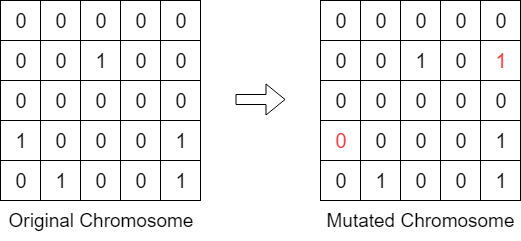
\includegraphics[width=100mm]{Figures/mutSmall.png}
        \caption{Mutation of a chromosome from the second generation}
        \label{mutSmall}
    \end{figure}
    
    Next, chromosomes produced in crossover have high chances of being infeasible thus needed to be repaired. Table \ref{repair1}, \ref{repair2} and \ref{repair3} list all the repaired infeasible chromosomes from the newly created generation.
    
    \begin{table}[h]
        \centering
        \begin{tabular}{|c|c|c|c|}
        \hline
       \textbf{Original} & \textbf{Repaired} & \textbf{Original} & \textbf{Repaired} \\ 
       \textbf{Chromosome} & \textbf{Chromosome} & \textbf{Chromosome} & \textbf{Chromosome} \\
       \hline
           $34th : \begin{bmatrix}
                0 & 1 & 0 & 0 & 0 \\
                1 & 0 & 0 & 0 & 0 \\
                0 & 0 & 0 & 0 & 0 \\
                0 & 0 & 1 & 0 & 0 \\
                0 & 0 & 0 & 1 & 0
            \end{bmatrix}
            $&
            $\begin{bmatrix}
                0 & 1 & 0 & 0 & 0 \\
                1 & 0 & 0 & 0 & 0 \\
                0 & 0 & 0 & 0 & 0 \\
                0 & 0 & 1 & 0 & 0 \\
                0 & 0 & 1 & 1 & 0
            \end{bmatrix}
            $&
            $35th : \begin{bmatrix}
                0 & 0 & 0 & 0 & 0 \\
                0 & 1 & 1 & 0 & 0 \\
                0 & 0 & 0 & 0 & 0 \\
                0 & 0 & 0 & 0 & 1 \\
                1 & 1 & 0 & 0 & 1
            \end{bmatrix}
            $&
            $\begin{bmatrix}
                0 & 0 & 0 & 0 & 0 \\
                0 & 1 & 1 & 0 & 0 \\
                0 & 0 & 0 & 0 & 0 \\
                0 & 0 & 0 & 0 & 1 \\
                1 & 0 & 0 & 0 & 1
            \end{bmatrix}
            $\\
            \hline
           $36th : \begin{bmatrix}
                0 & 1 & 1 & 0 & 0 \\
                0 & 0 & 0 & 0 & 0 \\
                0 & 0 & 0 & 0 & 0 \\
                0 & 0 & 1 & 0 & 1 \\
                0 & 0 & 0 & 0 & 0
            \end{bmatrix}
            $&
            $\begin{bmatrix}
                0 & 1 & 1 & 0 & 0 \\
                0 & 0 & 0 & 0 & 0 \\
                0 & 0 & 0 & 0 & 0 \\
                0 & 0 & 1 & 0 & 1 \\
                1 & 0 & 0 & 0 & 0
            \end{bmatrix}
            $&
            $37th : \begin{bmatrix}
                0 & 0 & 0 & 0 & 1 \\
                1 & 0 & 0 & 1 & 0 \\
                1 & 0 & 0 & 0 & 0 \\
                0 & 0 & 1 & 0 & 0 \\
                0 & 0 & 0 & 1 & 0
            \end{bmatrix}
            $&
            $\begin{bmatrix}
                0 & 0 & 0 & 0 & 1 \\
                1 & 0 & 0 & 0 & 0 \\
                1 & 0 & 0 & 0 & 0 \\
                0 & 0 & 1 & 0 & 0 \\
                0 & 0 & 0 & 1 & 0
            \end{bmatrix}
            $\\
            \hline
           $38th : \begin{bmatrix}
                0 & 1 & 0 & 0 & 0 \\
                1 & 1 & 0 & 0 & 1 \\
                0 & 0 & 0 & 0 & 0 \\
                0 & 0 & 0 & 0 & 0 \\
                1 & 0 & 0 & 1 & 0
            \end{bmatrix}
            $&
            $\begin{bmatrix}
                0 & 1 & 0 & 0 & 0 \\
                1 & 1 & 0 & 0 & 1 \\
                0 & 0 & 0 & 0 & 0 \\
                0 & 0 & 0 & 0 & 0 \\
                1 & 0 & 0 & 0 & 0
            \end{bmatrix}
            $&
            $39th : \begin{bmatrix}
                0 & 0 & 0 & 0 & 0 \\
                0 & 0 & 0 & 0 & 0 \\
                0 & 1 & 0 & 0 & 0 \\
                1 & 0 & 0 & 1 & 0 \\
                0 & 0 & 0 & 0 & 1
            \end{bmatrix}
            $&
            $\begin{bmatrix}
                0 & 0 & 1 & 0 & 0 \\
                0 & 0 & 0 & 0 & 0 \\
                0 & 1 & 0 & 0 & 0 \\
                1 & 0 & 0 & 1 & 0 \\
                0 & 0 & 0 & 0 & 1
            \end{bmatrix}
            $\\
            \hline
           $40th : \begin{bmatrix}
                1 & 0 & 0 & 0 & 0 \\
                0 & 0 & 0 & 0 & 0 \\
                0 & 1 & 0 & 0 & 0 \\
                0 & 0 & 0 & 0 & 0 \\
                0 & 0 & 0 & 1 & 1
            \end{bmatrix}
            $&
            $\begin{bmatrix}
                1 & 0 & 0 & 0 & 0 \\
                0 & 0 & 1 & 0 & 0 \\
                0 & 1 & 0 & 0 & 0 \\
                0 & 0 & 0 & 0 & 0 \\
                0 & 0 & 0 & 1 & 1
            \end{bmatrix}
            $&
            $41th : \begin{bmatrix}
                0 & 0 & 0 & 1 & 0 \\
                0 & 0 & 0 & 0 & 1 \\
                1 & 0 & 0 & 1 & 0 \\
                0 & 0 & 0 & 0 & 0 \\
                1 & 0 & 0 & 1 & 0
            \end{bmatrix}
            $&
            $\begin{bmatrix}
                0 & 0 & 0 & 1 & 0 \\
                0 & 0 & 0 & 0 & 1 \\
                0 & 0 & 0 & 1 & 0 \\
                0 & 0 & 0 & 0 & 0 \\
                1 & 0 & 0 & 1 & 0
            \end{bmatrix}
            $\\
            \hline
           $42th : \begin{bmatrix}
                0 & 1 & 0 & 0 & 0 \\
                0 & 0 & 0 & 0 & 1 \\
                0 & 0 & 1 & 0 & 0 \\
                0 & 0 & 0 & 0 & 0 \\
                1 & 0 & 1 & 0 & 1
            \end{bmatrix}
            $&
            $\begin{bmatrix}
                0 & 1 & 0 & 0 & 0 \\
                0 & 0 & 0 & 0 & 1 \\
                0 & 0 & 1 & 0 & 0 \\
                0 & 0 & 0 & 0 & 0 \\
                1 & 0 & 0 & 0 & 1
            \end{bmatrix}
            $&
            $43th : \begin{bmatrix}
                0 & 0 & 1 & 0 & 1 \\
                0 & 0 & 0 & 0 & 0 \\
                0 & 0 & 0 & 1 & 0 \\
                0 & 0 & 0 & 0 & 1 \\
                0 & 0 & 0 & 0 & 0
            \end{bmatrix}
            $&
            $\begin{bmatrix}
                0 & 0 & 1 & 0 & 1 \\
                0 & 0 & 0 & 0 & 0 \\
                0 & 0 & 0 & 1 & 0 \\
                0 & 0 & 0 & 0 & 1 \\
                1 & 0 & 0 & 0 & 0
            \end{bmatrix}
            $\\
            \hline
           $44th : \begin{bmatrix}
                0 & 1 & 0 & 0 & 0 \\
                0 & 0 & 0 & 0 & 0 \\
                1 & 0 & 0 & 0 & 0 \\
                0 & 0 & 0 & 0 & 0 \\
                0 & 0 & 0 & 0 & 1
            \end{bmatrix}
            $&
            $\begin{bmatrix}
                0 & 1 & 0 & 0 & 0 \\
                0 & 0 & 0 & 0 & 0 \\
                1 & 0 & 1 & 0 & 0 \\
                0 & 0 & 0 & 0 & 0 \\
                0 & 1 & 0 & 0 & 1
            \end{bmatrix}
            $&
            $45th : \begin{bmatrix}
                0 & 1 & 0 & 0 & 1 \\
                0 & 0 & 0 & 0 & 0 \\
                0 & 1 & 1 & 0 & 0 \\
                0 & 0 & 0 & 0 & 0 \\
                1 & 0 & 1 & 0 & 1
            \end{bmatrix}
            $&
            $\begin{bmatrix}
                0 & 1 & 0 & 0 & 0 \\
                0 & 0 & 0 & 0 & 0 \\
                0 & 1 & 0 & 0 & 0 \\
                0 & 0 & 0 & 0 & 0 \\
                1 & 0 & 1 & 0 & 1
            \end{bmatrix}
            $\\
            \hline
           $46th : \begin{bmatrix}
                0 & 0 & 0 & 0 & 0 \\
                0 & 0 & 0 & 0 & 1 \\
                0 & 0 & 1 & 0 & 0 \\
                0 & 0 & 0 & 0 & 0 \\
                0 & 0 & 0 & 1 & 1
            \end{bmatrix}
            $&
            $\begin{bmatrix}
                0 & 0 & 0 & 0 & 0 \\
                0 & 0 & 0 & 0 & 1 \\
                0 & 1 & 0 & 1 & 0 \\
                0 & 0 & 0 & 0 & 0 \\
                0 & 0 & 0 & 1 & 1
            \end{bmatrix}
            $&
            $47th : \begin{bmatrix}
                1 & 0 & 0 & 1 & 0 \\
                0 & 0 & 0 & 0 & 0 \\
                1 & 0 & 0 & 1 & 0 \\
                0 & 0 & 0 & 0 & 0 \\
                1 & 0 & 0 & 1 & 0
            \end{bmatrix}
            $&
            $\begin{bmatrix}
                1 & 0 & 0 & 1 & 0 \\
                0 & 0 & 0 & 0 & 0 \\
                0 & 0 & 0 & 1 & 0 \\
                0 & 0 & 0 & 0 & 0 \\
                1 & 0 & 0 & 1 & 0
            \end{bmatrix}
            $\\
            \hline
           $50th : \begin{bmatrix}
                0 & 0 & 0 & 0 & 0 \\
                0 & 0 & 0 & 0 & 0 \\
                1 & 1 & 0 & 0 & 0 \\
                0 & 0 & 1 & 0 & 0 \\
                0 & 0 & 0 & 0 & 0
            \end{bmatrix}
            $&
            $\begin{bmatrix}
                0 & 0 & 0 & 0 & 1 \\
                0 & 0 & 0 & 0 & 0 \\
                1 & 1 & 0 & 0 & 0 \\
                0 & 0 & 1 & 1 & 0 \\
                0 & 0 & 0 & 0 & 0
            \end{bmatrix}
            $&
            $51th : \begin{bmatrix}
                0 & 1 & 0 & 0 & 0 \\
                0 & 1 & 0 & 1 & 0 \\
                1 & 1 & 0 & 0 & 0 \\
                0 & 0 & 0 & 0 & 0 \\
                0 & 0 & 1 & 0 & 1
            \end{bmatrix}
            $&
            $\begin{bmatrix}
                0 & 1 & 0 & 0 & 0 \\
                0 & 0 & 0 & 1 & 0 \\
                0 & 1 & 0 & 0 & 0 \\
                0 & 0 & 0 & 0 & 0 \\
                0 & 0 & 1 & 0 & 1
            \end{bmatrix}
            $\\
            \hline
        \end{tabular}
        \caption{Chromosomes 34 to 51 before and after the repair}
        \label{repair1}
    \end{table}
    
    \begin{table}[h]
        \centering
        \begin{tabular}{|c|c|c|c|}
        \hline
       \textbf{Original} & \textbf{Repaired} & \textbf{Original} & \textbf{Repaired} \\         \textbf{Chromosome} & \textbf{Chromosome} & \textbf{Chromosome} & \textbf{Chromosome} \\
       \hline
       $54th : \begin{bmatrix}
                0 & 0 & 0 & 0 & 0 \\
                0 & 0 & 0 & 1 & 0 \\
                0 & 0 & 0 & 0 & 1 \\
                0 & 0 & 0 & 0 & 0 \\
                1 & 0 & 0 & 0 & 1
            \end{bmatrix}
            $&
            $\begin{bmatrix}
                0 & 0 & 0 & 0 & 1 \\
                0 & 0 & 0 & 1 & 0 \\
                0 & 0 & 0 & 0 & 1 \\
                0 & 0 & 0 & 0 & 0 \\
                1 & 0 & 0 & 0 & 1
            \end{bmatrix}
            $&
            $55th : \begin{bmatrix}
                0 & 0 & 0 & 0 & 1 \\
                1 & 0 & 0 & 0 & 0 \\
                0 & 0 & 0 & 0 & 0 \\
                0 & 0 & 1 & 1 & 1 \\
                0 & 0 & 0 & 1 & 0
            \end{bmatrix}
            $&
            $\begin{bmatrix}
                0 & 0 & 0 & 0 & 0 \\
                1 & 0 & 0 & 0 & 0 \\
                0 & 0 & 0 & 0 & 0 \\
                0 & 0 & 1 & 1 & 1 \\
                0 & 0 & 0 & 1 & 0
            \end{bmatrix}
            $\\\hline
           $56th : \begin{bmatrix}
                1 & 0 & 0 & 0 & 0 \\
                0 & 0 & 0 & 0 & 1 \\
                0 & 1 & 0 & 0 & 0 \\
                0 & 0 & 0 & 1 & 0 \\
                1 & 0 & 0 & 0 & 1
            \end{bmatrix}
            $&
            $\begin{bmatrix}
                1 & 0 & 0 & 0 & 0 \\
                0 & 0 & 0 & 0 & 1 \\
                0 & 1 & 0 & 0 & 0 \\
                0 & 0 & 0 & 0 & 0 \\
                1 & 0 & 0 & 0 & 1
            \end{bmatrix}
            $&
            $57th : \begin{bmatrix}
                1 & 0 & 0 & 0 & 0 \\
                1 & 0 & 0 & 0 & 0 \\
                0 & 0 & 0 & 0 & 0 \\
                0 & 0 & 0 & 0 & 0 \\
                1 & 0 & 0 & 1 & 0
            \end{bmatrix}
            $&
            $\begin{bmatrix}
                1 & 0 & 0 & 0 & 0 \\
                1 & 0 & 0 & 0 & 0 \\
                0 & 0 & 1 & 0 & 0 \\
                0 & 0 & 0 & 0 & 0 \\
                1 & 0 & 0 & 1 & 0
            \end{bmatrix}
            $\\
            \hline
           $60th : \begin{bmatrix}
                0 & 1 & 0 & 0 & 1 \\
                1 & 0 & 0 & 0 & 0 \\
                0 & 1 & 0 & 0 & 0 \\
                0 & 0 & 1 & 0 & 1 \\
                0 & 0 & 0 & 1 & 0
            \end{bmatrix}
            $&
            $\begin{bmatrix}
                0 & 1 & 0 & 0 & 1 \\
                1 & 0 & 0 & 0 & 0 \\
                0 & 0 & 0 & 0 & 0 \\
                0 & 0 & 1 & 0 & 0 \\
                0 & 0 & 0 & 1 & 0
            \end{bmatrix}
            $&
            $61th : \begin{bmatrix}
                0 & 0 & 0 & 0 & 0 \\
                0 & 0 & 0 & 0 & 0 \\
                1 & 0 & 0 & 0 & 0 \\
                0 & 0 & 0 & 0 & 0 \\
                0 & 0 & 1 & 0 & 1
            \end{bmatrix}
            $&
            $\begin{bmatrix}
                0 & 0 & 0 & 0 & 0 \\
                0 & 0 & 0 & 0 & 0 \\
                1 & 0 & 0 & 1 & 0 \\
                1 & 0 & 0 & 0 & 0 \\
                0 & 0 & 1 & 0 & 1
            \end{bmatrix}
            $\\
            \hline
           $62th : \begin{bmatrix}
                0 & 1 & 1 & 1 & 0 \\
                0 & 0 & 0 & 1 & 0 \\
                0 & 0 & 0 & 0 & 0 \\
                0 & 0 & 1 & 1 & 0 \\
                0 & 0 & 0 & 0 & 0
            \end{bmatrix}
            $&
            $\begin{bmatrix}
                0 & 1 & 0 & 1 & 0 \\
                0 & 0 & 0 & 1 & 0 \\
                0 & 0 & 0 & 0 & 0 \\
                0 & 0 & 1 & 1 & 0 \\
                0 & 0 & 0 & 0 & 0
            \end{bmatrix}
            $&
            $63th : \begin{bmatrix}
                1 & 0 & 0 & 0 & 0 \\
                0 & 0 & 0 & 0 & 0 \\
                1 & 0 & 0 & 0 & 0 \\
                0 & 0 & 1 & 0 & 0 \\
                1 & 0 & 0 & 0 & 0
            \end{bmatrix}
            $&
            $\begin{bmatrix}
                1 & 0 & 0 & 0 & 0 \\
                0 & 0 & 0 & 0 & 0 \\
                1 & 1 & 0 & 0 & 0 \\
                0 & 0 & 1 & 0 & 0 \\
                1 & 0 & 0 & 0 & 0
            \end{bmatrix}
            $\\
            \hline
           $64th : \begin{bmatrix}
                0 & 1 & 0 & 0 & 0 \\
                0 & 0 & 1 & 1 & 0 \\
                0 & 0 & 0 & 0 & 0 \\
                0 & 0 & 0 & 0 & 0 \\
                0 & 0 & 1 & 0 & 0
            \end{bmatrix}
            $&
            $\begin{bmatrix}
                0 & 1 & 0 & 0 & 0 \\
                0 & 0 & 1 & 1 & 0 \\
                0 & 1 & 0 & 0 & 0 \\
                0 & 0 & 0 & 0 & 0 \\
                0 & 0 & 1 & 0 & 0
            \end{bmatrix}
            $&
            $65th : \begin{bmatrix}
                1 & 0 & 1 & 0 & 0 \\
                0 & 0 & 0 & 1 & 0 \\
                1 & 1 & 0 & 0 & 0 \\
                0 & 0 & 1 & 0 & 0 \\
                0 & 0 & 0 & 0 & 0
            \end{bmatrix}
            $&
            $\begin{bmatrix}
                1 & 0 & 1 & 0 & 0 \\
                0 & 0 & 0 & 1 & 0 \\
                0 & 1 & 0 & 0 & 0 \\
                0 & 0 & 1 & 0 & 0 \\
                0 & 0 & 0 & 0 & 0
            \end{bmatrix}
            $\\
            \hline
           $66th : \begin{bmatrix}
                0 & 0 & 0 & 1 & 0 \\
                0 & 0 & 0 & 0 & 0 \\
                0 & 0 & 0 & 1 & 0 \\
                0 & 0 & 1 & 0 & 0 \\
                0 & 0 & 0 & 0 & 1
            \end{bmatrix}
            $&
            $\begin{bmatrix}
                0 & 0 & 0 & 1 & 0 \\
                0 & 0 & 0 & 0 & 1 \\
                0 & 0 & 0 & 1 & 0 \\
                0 & 0 & 1 & 0 & 0 \\
                0 & 0 & 0 & 0 & 1
            \end{bmatrix}
            $&
            $67th : \begin{bmatrix}
                0 & 1 & 0 & 0 & 0 \\
                0 & 0 & 0 & 0 & 1 \\
                0 & 1 & 0 & 0 & 0 \\
                0 & 0 & 0 & 0 & 0 \\
                1 & 1 & 0 & 0 & 1
            \end{bmatrix}
            $&
            $\begin{bmatrix}
                0 & 0 & 0 & 0 & 0 \\
                0 & 0 & 0 & 0 & 1 \\
                0 & 1 & 0 & 0 & 0 \\
                0 & 0 & 0 & 0 & 0 \\
                1 & 1 & 0 & 0 & 1
            \end{bmatrix}
            $\\
            \hline
           $68th : \begin{bmatrix}
                0 & 0 & 0 & 1 & 0 \\
                0 & 0 & 1 & 0 & 0 \\
                1 & 0 & 0 & 1 & 1 \\
                0 & 0 & 0 & 0 & 0 \\
                0 & 0 & 0 & 1 & 0
            \end{bmatrix}
            $&
            $\begin{bmatrix}
                0 & 0 & 0 & 1 & 0 \\
                0 & 0 & 1 & 0 & 0 \\
                1 & 0 & 0 & 1 & 0 \\
                0 & 0 & 0 & 0 & 0 \\
                0 & 0 & 0 & 1 & 0
            \end{bmatrix}
            $&
            $69th : \begin{bmatrix}
                0 & 0 & 0 & 1 & 0 \\
                0 & 0 & 0 & 0 & 1 \\
                0 & 0 & 0 & 0 & 0 \\
                0 & 0 & 0 & 0 & 0 \\
                1 & 0 & 0 & 1 & 0
            \end{bmatrix}
            $&
            $\begin{bmatrix}
                0 & 0 & 0 & 1 & 0 \\
                0 & 0 & 0 & 0 & 1 \\
                0 & 0 & 0 & 0 & 1 \\
                0 & 0 & 0 & 0 & 0 \\
                1 & 0 & 0 & 1 & 0
            \end{bmatrix}
            $\\
            \hline
           $70th : \begin{bmatrix}
                0 & 1 & 0 & 1 & 0 \\
                0 & 0 & 0 & 0 & 0 \\
                0 & 1 & 0 & 0 & 0 \\
                0 & 0 & 1 & 0 & 0 \\
                1 & 0 & 0 & 0 & 1
            \end{bmatrix}
            $&
            $\begin{bmatrix}
                0 & 1 & 0 & 1 & 0 \\
                0 & 0 & 0 & 0 & 0 \\
                0 & 1 & 0 & 0 & 0 \\
                0 & 0 & 1 & 0 & 0 \\
                0 & 0 & 0 & 0 & 1
            \end{bmatrix}
            $&
            $71th : \begin{bmatrix}
                0 & 0 & 1 & 0 & 0 \\
                0 & 0 & 0 & 0 & 1 \\
                0 & 0 & 0 & 0 & 0 \\
                0 & 0 & 1 & 0 & 0 \\
                0 & 0 & 1 & 0 & 0
            \end{bmatrix}
            $&
            $\begin{bmatrix}
                0 & 0 & 1 & 0 & 0 \\
                0 & 0 & 0 & 0 & 1 \\
                0 & 1 & 0 & 0 & 0 \\
                0 & 0 & 1 & 0 & 0 \\
                0 & 0 & 1 & 0 & 0
            \end{bmatrix}
            $\\
            \hline
           $76th : \begin{bmatrix}
                0 & 0 & 0 & 0 & 0 \\
                0 & 1 & 0 & 0 & 0 \\
                0 & 0 & 0 & 0 & 1 \\
                0 & 0 & 0 & 0 & 1 \\
                1 & 1 & 0 & 0 & 1
            \end{bmatrix}
            $&
            $\begin{bmatrix}
                0 & 0 & 0 & 0 & 0 \\
                0 & 1 & 0 & 0 & 0 \\
                0 & 0 & 0 & 0 & 1 \\
                0 & 0 & 0 & 0 & 0 \\
                1 & 1 & 0 & 0 & 1
            \end{bmatrix}
            $&
            $77th : \begin{bmatrix}
                0 & 1 & 0 & 0 & 0 \\
                1 & 0 & 1 & 0 & 0 \\
                0 & 0 & 0 & 0 & 0 \\
                0 & 1 & 0 & 0 & 0 \\
                0 & 0 & 0 & 0 & 0
            \end{bmatrix}
            $&
            $\begin{bmatrix}
                0 & 1 & 0 & 0 & 0 \\
                1 & 0 & 1 & 0 & 0 \\
                1 & 0 & 0 & 0 & 0 \\
                0 & 1 & 0 & 0 & 0 \\
                0 & 0 & 0 & 0 & 0
            \end{bmatrix}
            $\\
            \hline
           
        \end{tabular}
        \caption{Chromosome 54 to 77 before and after the repair}
        \label{repair2}
    \end{table}

    \begin{table}[h]
        \centering
        \begin{tabular}{|c|c|c|c|}
        \hline
       \textbf{Original} & \textbf{Repaired} & \textbf{Original} & \textbf{Repaired} \\         \textbf{Chromosome} & \textbf{Chromosome} & \textbf{Chromosome} & \textbf{Chromosome} \\
       \hline
        $80th : \begin{bmatrix}
                0 & 0 & 0 & 0 & 0 \\
                1 & 0 & 1 & 0 & 0 \\
                0 & 0 & 0 & 0 & 0 \\
                0 & 1 & 1 & 0 & 0 \\
                0 & 0 & 1 & 1 & 0
            \end{bmatrix}
            $&
            $\begin{bmatrix}
                0 & 0 & 0 & 0 & 0 \\
                1 & 0 & 0 & 0 & 0 \\
                0 & 0 & 0 & 0 & 0 \\
                0 & 1 & 1 & 0 & 0 \\
                0 & 0 & 1 & 1 & 0
            \end{bmatrix}
            $&
            $81th : \begin{bmatrix}
                0 & 0 & 0 & 1 & 1 \\
                0 & 0 & 0 & 0 & 0 \\
                1 & 0 & 0 & 0 & 0 \\
                0 & 0 & 0 & 0 & 1 \\
                0 & 0 & 0 & 0 & 0
            \end{bmatrix}
            $&
            $\begin{bmatrix}
                0 & 0 & 0 & 1 & 1 \\
                0 & 0 & 0 & 0 & 0 \\
                1 & 0 & 0 & 0 & 0 \\
                0 & 0 & 0 & 0 & 1 \\
                0 & 0 & 0 & 0 & 0
            \end{bmatrix}
            $\\
            \hline
            $84th :\begin{bmatrix}
                1 & 1 & 0 & 0 & 0 \\
                0 & 0 & 0 & 0 & 0 \\
                0 & 1 & 0 & 0 & 0 \\
                0 & 0 & 0 & 0 & 0 \\
                1 & 0 & 1 & 0 & 1
            \end{bmatrix}
            $&
            $\begin{bmatrix}
                1 & 1 & 0 & 0 & 0 \\
                0 & 0 & 0 & 0 & 0 \\
                0 & 0 & 0 & 0 & 0 \\
                0 & 0 & 0 & 0 & 0 \\
                1 & 0 & 1 & 0 & 1
            \end{bmatrix}
            $&
            $85th :\begin{bmatrix}
                0 & 0 & 0 & 0 & 1 \\
                0 & 0 & 0 & 0 & 0 \\
                1 & 0 & 0 & 0 & 0 \\
                0 & 0 & 0 & 0 & 0 \\
                1 & 0 & 0 & 1 & 0
            \end{bmatrix}
            $&
            $\begin{bmatrix}
                0 & 0 & 0 & 1 & 1 \\
                0 & 0 & 0 & 0 & 0 \\
                1 & 0 & 0 & 0 & 0 \\
                0 & 0 & 0 & 0 & 0 \\
                1 & 0 & 0 & 1 & 0
            \end{bmatrix}
            $\\
            \hline
            $88th :\begin{bmatrix}
                1 & 0 & 0 & 0 & 1 \\
                0 & 0 & 0 & 0 & 0 \\
                1 & 0 & 0 & 0 & 1 \\
                1 & 0 & 0 & 0 & 0 \\
                0 & 0 & 1 & 1 & 0
            \end{bmatrix}
            $&
            $\begin{bmatrix}
                0 & 0 & 0 & 0 & 1 \\
                0 & 0 & 0 & 0 & 0 \\
                1 & 0 & 0 & 0 & 1 \\
                1 & 0 & 0 & 0 & 0 \\
                0 & 0 & 0 & 1 & 0
            \end{bmatrix}
            $&
            $89th :\begin{bmatrix}
                0 & 0 & 0 & 0 & 0 \\
                0 & 0 & 0 & 0 & 0 \\
                1 & 0 & 0 & 0 & 0 \\
                1 & 0 & 0 & 1 & 0 \\
                0 & 0 & 0 & 0 & 0
            \end{bmatrix}
            $&
            $\begin{bmatrix}
                0 & 0 & 0 & 0 & 0 \\
                0 & 0 & 0 & 0 & 0 \\
                1 & 0 & 0 & 0 & 0 \\
                1 & 0 & 0 & 1 & 1 \\
                1 & 0 & 0 & 0 & 0
            \end{bmatrix}
            $\\
            \hline
            $90th :\begin{bmatrix}
                0 & 1 & 0 & 0 & 0 \\
                0 & 0 & 0 & 0 & 0 \\
                0 & 1 & 0 & 0 & 0 \\
                0 & 0 & 1 & 0 & 0 \\
                1 & 0 & 0 & 1 & 1
            \end{bmatrix}
            $&
            $\begin{bmatrix}
                0 & 1 & 0 & 0 & 0 \\
                0 & 0 & 0 & 0 & 0 \\
                0 & 1 & 0 & 0 & 0 \\
                0 & 0 & 1 & 0 & 0 \\
                1 & 0 & 0 & 0 & 1
            \end{bmatrix}
            $&
            $91st :\begin{bmatrix}
                1 & 0 & 0 & 1 & 0 \\
                0 & 0 & 0 & 0 & 0 \\
                0 & 1 & 0 & 0 & 0 \\
                0 & 0 & 0 & 0 & 0 \\
                0 & 0 & 0 & 0 & 1
            \end{bmatrix}
            $&
            $\begin{bmatrix}
                1 & 0 & 0 & 1 & 1 \\
                0 & 0 & 0 & 0 & 0 \\
                0 & 1 & 0 & 0 & 0 \\
                0 & 0 & 0 & 0 & 0 \\
                0 & 0 & 0 & 0 & 1
            \end{bmatrix}
            $\\
            \hline
            $94th :\begin{bmatrix}
                1 & 1 & 0 & 0 & 0 \\
                0 & 0 & 0 & 0 & 0 \\
                0 & 0 & 0 & 0 & 0 \\
                0 & 0 & 0 & 0 & 0 \\
                1 & 0 & 0 & 0 & 0
            \end{bmatrix}
            $&
            $\begin{bmatrix}
                1 & 1 & 0 & 0 & 0 \\
                1 & 0 & 0 & 0 & 0 \\
                0 & 0 & 0 & 0 & 1 \\
                0 & 0 & 0 & 0 & 0 \\
                1 & 0 & 0 & 0 & 0
            \end{bmatrix}
            $&
            $95th :\begin{bmatrix}
                0 & 0 & 0 & 1 & 1 \\
                0 & 0 & 0 & 0 & 0 \\
                0 & 0 & 1 & 0 & 0 \\
                0 & 0 & 1 & 1 & 0 \\
                1 & 0 & 0 & 0 & 1
            \end{bmatrix}
            $&
            $\begin{bmatrix}
                0 & 0 & 0 & 0 & 1 \\
                0 & 0 & 0 & 0 & 0 \\
                0 & 0 & 1 & 0 & 0 \\
                0 & 0 & 1 & 1 & 0 \\
                1 & 0 & 0 & 0 & 0
            \end{bmatrix}
            $\\
            \hline
            $96th :\begin{bmatrix}
                0 & 1 & 0 & 1 & 0 \\
                0 & 0 & 0 & 0 & 0 \\
                1 & 0 & 0 & 0 & 0 \\
                0 & 0 & 0 & 0 & 0 \\
                0 & 0 & 0 & 1 & 0
            \end{bmatrix}
            $&
            $\begin{bmatrix}
                1 & 1 & 0 & 1 & 0 \\
                0 & 0 & 0 & 0 & 0 \\
                1 & 0 & 0 & 0 & 0 \\
                0 & 0 & 0 & 0 & 0 \\
                0 & 0 & 0 & 1 & 0
            \end{bmatrix}
            $&
            $97th :\begin{bmatrix}
                0 & 0 & 0 & 0 & 1 \\
                0 & 0 & 0 & 0 & 1 \\
                0 & 0 & 1 & 1 & 0 \\
                0 & 0 & 0 & 0 & 0 \\
                1 & 0 & 0 & 0 & 1
            \end{bmatrix}
            $&
            $\begin{bmatrix}
                0 & 0 & 0 & 0 & 0 \\
                0 & 0 & 0 & 0 & 1 \\
                0 & 0 & 1 & 1 & 0 \\
                0 & 0 & 0 & 0 & 0 \\
                1 & 0 & 0 & 0 & 1
            \end{bmatrix}
            $\\
            \hline
            $98th :\begin{bmatrix}
                0 & 0 & 0 & 1 & 0 \\
                0 & 0 & 0 & 1 & 0 \\
                1 & 0 & 0 & 0 & 1 \\
                1 & 0 & 0 & 0 & 0 \\
                0 & 0 & 1 & 0 & 0
            \end{bmatrix}
            $&
            $\begin{bmatrix}
                0 & 0 & 0 & 1 & 0 \\
                0 & 0 & 0 & 0 & 0 \\
                1 & 0 & 0 & 0 & 1 \\
                1 & 0 & 0 & 0 & 0 \\
                0 & 0 & 1 & 0 & 0
            \end{bmatrix}
            $&
            $99th :\begin{bmatrix}
                0 & 1 & 0 & 0 & 0 \\
                0 & 0 & 0 & 0 & 0 \\
                0 & 0 & 0 & 0 & 0 \\
                1 & 0 & 0 & 1 & 0 \\
                0 & 0 & 1 & 0 & 0
            \end{bmatrix}
            $&
            $\begin{bmatrix}
                0 & 1 & 0 & 0 & 0 \\
                0 & 0 & 0 & 0 & 0 \\
                0 & 0 & 0 & 0 & 0 \\
                1 & 0 & 0 & 1 & 1 \\
                0 & 0 & 1 & 0 & 0
            \end{bmatrix}
            $\\
            \hline

            \end{tabular}
        \caption{Chromosome 80 to 99  before and after the repair}
        \label{repair3}
    \end{table}
    
    Having all infeasible chromosomes repaired, the new generation will now undergo the same process as the last generation. It is found that the most fit chromosome from generation and generation are the same which has a fitness value of $0.001952\;kW^{-1}$. However, comparing the average fitness of generation 1 which is $0.002005\;kW^{-1}$ to average fitness of generation 2 which is $0.001989\;kW^{-1}$, the average fitness of generation 2 is better than the previous generation proving that in every generation the collective fitness of the chromosomes improved.

    The steps for each generation are repeated until the individuals of the whole generation converged to a single chromosome. Table \ref{summaryGASmall} shows the average fitness and the fitness of the most fit chromosome of each generation.
    
    \begin{table}[]
        \centering
        \begin{tabular}{|ccc|ccc|}
            \hline
            \multirow{2}{*}{\textbf{Gen}} & \multicolumn{2}{c|}{\textbf{Fitness Value ($kW^{-1}$)}} & \multirow{2}{*}{\textbf{Gen}} & \multicolumn{2}{c|}{\textbf{Fitness Value ($kW^{-1}$)}} \\ \cline{2-3} \cline{5-6} 
                                          & \textbf{Best}       & \textbf{Average}      &                               & \textbf{Best}       & \textbf{Average}      \\ \hline
            1                             & 0.001952            & 0.002005              & 10                            & 0.001952            & 0.001964              \\ \hline
            2                             & 0.001952            & 0.001989              & 11                            & 0.001952            & 0.001964              \\ \hline
            3                             & 0.001954            & 0.001987              & 12                            & 0.001952            & 0.001960              \\ \hline
            4                             & 0.001957            & 0.001985              & 13                            & 0.001952            & 0.001957              \\ \hline
            5                             & 0.001955            & 0.001981              & 14                            & 0.001952            & 0.001958              \\ \hline
            6                             & 0.001955            & 0.001977              & 15                            & 0.001952            & 0.001955              \\ \hline
            7                             & 0.001954            & 0.001975              & 16                            & 0.001952            & 0.001953              \\ \hline
            8                             & 0.001954            & 0.001968              & 17                            & 0.001952            & 0.001952              \\ \hline
            9                             & 0.001954            & 0.001968              &                               &                     &                       \\ \hline
        \end{tabular}
        \caption{Average fitness and fitness of most fit chromosome of each generation for wind turbine siting of 5 wind turbines on a $1km$ by $1km$ wind farm with multiple wind direction}
        \label{summaryGASmall}
    \end{table}
    
    After the first phase of the algorithm, the BRCGA gave the most fit chromosome with fitness of $0.001952\;kW^{-1}$ with the chromosome wind farm model shown in figure \ref{phase1chromSmall}.
    
    \begin{figure}[h]
        \centering
        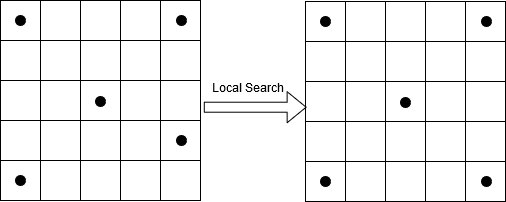
\includegraphics[width=\linewidth]{Figures/phase1chromSmall.png}
        \caption{Wind farm model of the most optimal siting of 5 wind turbines on a $1\;km$ by $1\;km$ wind farm with multiple wind direction using the first phase of the proposed algorithm (left) and the same wind farm model after applying local search (right)}
        \label{phase1chromSmall}
    \end{figure}
    
    For the second phase of the proposed algorithm, the first iteration of the local search gives the list all the neighboring solutions of the solution from the BRCGA. Each wind turbine will move to at most 8 adjacent location and check whether the fitness has improved. From figure \ref{phase1chromSmall}, the wind turbine located at $(0,0)$ can move to locations $(0,1)$, $(1,0)$ and $(1,1)$ of wind farm shown on the left which can result to three neighboring solutions. For the current state of the wind farm shown on the left in figure \ref{phase1chromSmall}, there were 22 neighboring solutions for the first iteration of the local search. A more fit solution is found when the wind turbine located at $(4,3)$ moved to an adjacent location in $(4,4)$, having a fitness value of $0.001948\;kW^{-1}$. This is now the current solution for the problem. However, the second iteration of the local search didn't find a more fit solution, hence marks the termination of the search. The final solution is shown on the right in Figure \ref{phase1chromSmall}.